% Template for a Computer Science Tripos Part II project dissertation
\documentclass[12pt,a4paper,twoside,openright]{report}
\usepackage[pdfborder={0 0 0}]{hyperref}    % turns references into hyperlinks
\usepackage[margin=25mm]{geometry}  % adjusts page layout
\usepackage{graphicx, color}  % allows inclusion of PDF, PNG and JPG images
\usepackage{verbatim}
\usepackage{docmute}   % only needed to allow inclusion of proposal.tex
\usepackage{dsfont, amsmath, textcomp}
\usepackage{pdfpages}
\usepackage{listings}
\usepackage{booktabs}
\usepackage[table,xcdraw]{xcolor}
\definecolor{mygray}{rgb}{0.8,0.8,0.8}
\usepackage{caption,inconsolata}
\DeclareCaptionFont{black}{\color{black}}
\DeclareCaptionFormat{listing}{%
  \parbox{\textwidth}{\colorbox{white}{\parbox{\textwidth}{#1#2#3}}\vskip-4pt}}
\captionsetup[lstlisting]{format=listing,labelfont=black,textfont=black}
\lstset{frame=tlrb,xleftmargin=\fboxsep,xrightmargin=-\fboxsep,basicstyle=\ttfamily \footnotesize,breaklines=true}
\usepackage{multicol}
\usepackage{multirow}
\usepackage[symbol]{footmisc}
\usepackage{float}


\raggedbottom                           % try to avoid widows and orphans
\sloppy
\clubpenalty1000%
\widowpenalty1000%

% \usepackage[utf8]{inputenc}
% \usepackage[english]{babel}
% \usepackage[backend=biber, style=alphabetic, sorting=ynt]{biblatex}

% \addbibresource{refs.bib}

\renewcommand{\baselinestretch}{1.1}    % adjust line spacing to make

%###########################################################################
\newcommand{\projectTitle}{Investigating the effect of \\
 & Translation Quality on Summarization Quality}                                        % more readable
 
 \newcommand{\red}[1]{\textcolor{red}{#1}}
 \newcommand{\changedFont}[1]{{\fontfamily{qcr}\selectfont #1}}
 \newcommand{\fone}{$F_1$}
 
 \newenvironment{specialfootnote}
    {
    \renewcommand*{\thefootnote}{\fnsymbol{footnote}}
    }
    {
    \renewcommand*{\thefootnote}{\arabic{footnote}}
    }
 
%  \newcommand{\specialfootnotetext}[2]{
%  \renewcommand*{\thefootnote}{\fnsymbol{footnote}}
%  \footnotetext[#1]{#2}
%  \renewcommand*{\thefootnote}{\arabic{footnote}}
%  }
 
%  \newcommand{\specialfootnotemark}[1]{
%  \renewcommand*{\thefootnote}{\fnsymbol{footnote}}
%  \footnotemark[#1]
%  \renewcommand*{\thefootnote}{\arabic{footnote}}
%  }

 
 %###############################################################

\begin{document}
 \renewcommand*{\thefootnote}{\arabic{footnote}}
\pagenumbering{roman}
\bibliographystyle{plain}


%%%%%%%%%%%%%%%%%%%%%%%%%%%%%%%%%%%%%%%%%%%%%%%%%%%%%%%%%%%%%%%%%%%%%%%%
% Title


\pagestyle{empty}

\rightline{\LARGE \textbf{Anish Das}}

\vspace*{60mm}
\begin{center}
\Huge
\textbf{Investigating the effect of  Translation Quality on Summarization Quality}\\
Computer Science Tripos -- Part II\\[5mm]
Trinity Hall \\[5mm]
\today  % today's date
\end{center}

%%%%%%%%%%%%%%%%%%%%%%%%%%%%%%%%%%%%%%%%%%%%%%%%%%%%%%%%%%%%%%%%%%%%%%%%%%%%%%
% Proforma, table of contents and list of figures

\pagestyle{plain}

\chapter*{Proforma}

{\large
\begin{tabular}{ll}
Name:               & \bf Anish Das                      \\
College:            & \bf Trinity Hall                     \\
Project Title:      &  \projectTitle \\
Examination:        & \bf Computer Science Tripos -- Part II, June 2021  \\
Word Count:         & \bf \textcolor{red}{8266\footnotemark[1]
                      (well less than the 12000 limit)}  \\
Project Originator: & Dr Andrew Caines                  \\
Supervisor:         & Dr Andrew Caines \& Dr Zheng Yuan                   \\ 
\end{tabular}
}
\footnotetext[1]{This word count was computed
by the inbuilt word counter in OverLeaf}

\stepcounter{footnote}


\section*{Original Aims of the Project}

% \red{these need work}\\
To investigate the effect of translation quality on summarization quality. To train Neural Machine Translation (NMT) models using the Transformer architecture for multiple languages and then applying a pre-trained state-of-the-art summarization model to the translations produced by the models. To find the correlation between the BLEU scores (translation metric) and the ROUGE scores (summarization metric). 

% \red{[Finally, to try a different architecture for faster training of language models.]}

% To write a demonstration dissertation\footnote{A normal footnote without the
% complication of being in a table.} using \LaTeX\ to save
% student's time when writing their own dissertations. The dissertation
% should illustrate how to use the more common \LaTeX\ constructs. It
% should include pictures and diagrams to show how these can be
% incorporated into the dissertation.  It should contain the entire
% \LaTeX\ source of the dissertation and the makefile.  It should
% explain how to construct an MSDOS disk of the dissertation in
% Postscript format that can be used by the book shop for printing, and,
% finally, it should have the prescribed layout and format of a diploma
% dissertation.


\section*{Work Completed}
\red{needs work}\\
The Transformer architecture was built from scratch and has been used to create multiple translation models. Translation models have been used to translate the documents in the evaluation GV-crowd/snippet dataset from \cite{nguyen-daume-iii-2019-global}. The translated sentences were then summarized. The BLEU and ROUGE metrics were calculated along with qualitative comparison of the two scores.

\section*{Special Difficulties}
No special difficulties were encountered. 


% \red{Learning how to training Transformers is a difficult task that requires proper care towards various factors. 
% And having to work remotely for the entire year.} 
 
\newpage
\section*{Declaration}

I, Anish Das of Trinity Hall, being a candidate for Part II of the Computer Science Tripos, hereby declare 
that this dissertation and the work described in it are my own work,
unaided except as may be specified below, and that the dissertation
does not contain material that has already been used to any substantial
extent for a comparable purpose.

\bigskip
\leftline{Signed [signature]}

\medskip
\leftline{Date [date]}

\bigskip
\section*{Acknowledgements}

A huge thanks to my supervisors, Andrew Caines and Zheng Yuan, who's support throughout the project was immense. 


\tableofcontents

\listoffigures
\listoftables
% \lstlistoflistings



%%%%%%%%%%%%%%%%%%%%%%%%%%%%%%%%%%%%%%%%%%%%%%%%%%%%%%%%%%%%%%%%%%%%%%%
% now for the chapters

\pagestyle{headings}

\cleardoublepage\pagenumbering{arabic}

%%%%%%%%%%%%%%%%%%%%%%%%%%%%%%%%%%%%%%%%%%%%%%%%%%%%%%%%%%%%%%%%%%%%%%%%%%%%%%%%%%%%%%%%%%%%%%%%%%%%%
%%%%%%%%%%%%%%%%%%%%%%%%%%%%%%%%%%%%%%%%%%%%%%%%%%%%%%%%%%%%%%%%%%%%%%%%%%%%%%%%%%%%
\chapter{Introduction}
\label{intro}


Natural Language Processing (NLP) is a branch of Artificial Intelligence (A.I.) that seeks to bridge the gap between human communication and computer understanding. It incorporates and draws from many disciplines, including computer science and computational linguistics.  

\section{Motivation}
\label{motivation}

Within this vast and varied field of NLP lies the task of Cross-Lingual Summarization (CLS), which aims to produce a summary in one specific target language from a source document in different languages. This is an essential task because it will lift the language barrier, withholding easy access to information. However, the amount of textual data is immense and continues to grow day by day. Today it is impossible to keep up with it because a person simply does not have enough time to read it all. By summarizing the data, we trim it down to its most salient points, which can be consumed quickly, thus, allowing humans to consume a more significant amount of information and in a shorter amount of time.  Suppose it is deployed on a large scale. In that case, it will bring about an exponentially increase in the amount of information available to everyone and thus empower humans with the knowledge of the diverse world we live in today. 

\section{Project Focus}
\label{project-focus}

CLS has two main steps: first, Translating the source document into a target language and second, Summarizing the translated text. Since CLS is a two-step process, any errors in the first step will be carried forward and possibly amplified through the second step and end up in the resulting summary. Further, it is widely known that we require large sentence-aligned datasets to build good quality translation models. Language-pairs which have these large datasets are called high-resource and those without are called low-resource language-pairs. Therefore, translation models trained on low-resource language-pairs have quite a few inaccuracies in their translations. This raises the question of whether bad-quality translations will adversely affect the information content and the readability of the resultant summary. 

With this as a foundation, this project explores the effect of translation quality on summarisation quality, creating, training, and comparing translation models of differing quality. Translation models, like most machine learning systems, improve with more training and therefore, a model's features are check-pointed at regular intervals yielding model's of varying quality. 

\section{Related Work}
\label{related-work}
In the paper \cite{nguyen-daume-iii-2019-global}, the authors set out to build a for evaluating cross-lingual summarization methods. They used the Global Voices\footnote{https://globalvoices.org/} to collect news articles in 15 different languages. Moreover, they crowd-sourced human summarizations of the articles collected in English and web-scraped the \textit{"snippet"} summaries available on the website. Finally, they trained four translation models, two of which were trained on a large scale dataset and the other two using a much smaller dataset. They used the different sized datasets to vary the quality of the final translation models and compared the resultant translations' ROUGE scores. 

This project borrows from \cite{nguyen-daume-iii-2019-global}. Instead of using multiple language-pairs with different dataset sizes, this project considers multiple models of the same language pair and trained on the same dataset and only varying the time it has been trained. This project extends the investigation carried out by the authors, to compare multiple model's of the same language pair as opposed to across different language pairs with differing dataset size (resource availability). This idea was born from the intuition that some languages, and by extension their translations, may be less compressible to begin with. Therefore, to truly evaluate the effects of translation on summarization, we should minimize the number of confounding variables, and thus, check-point models during the training process after every epoch to use as a proxy for worse translation quality. 

The architecture used to implement the translation models is the Transformer architecture \cite{transformers}, details of its conception and implementation are detailed in the following chapters. Finally, transformers are a deep architecture which are over 200 megabytes in size, which leads to them being very unstable in the training process and the investigation carried out in the article \cite{training-tips} helped guide the training process to run without a hitch. 

\section{Organisation of this Document}
\label{doc-org}
As per the requirements for this dissertation, there are chapters dedicated to the Preparation, Implementation, Evaluation and finally, a chapter Concluding the project and dissertation. 

\textbf{Chapter \ref{preperation} \nameref{preperation} }describes the work undertaken before pogramming commenced and also aims to build the theoretical basis needed to understand this document. It begins with a description of the \nameref{starting-point} and moves on to explaining the terms used throughout. Further, it details the background knowledge acquired during the Step 1 of the software engineering process (Understanding the Core requirements and Feasibility Study). Finally, the project management decisions are stated which includes on the Functional \& Non-Functional Requirements; Datasets used for training \& evaluation; the tools used and the platform where the project was run. 

\textbf{Chapter \ref{implementation} \nameref{implementation}} details the crux of the project, i.e. is the implementation of the Translation system and evaluating the summaries produced. It begins with a description of the pre-processing steps utilized, followed by a fine-grained explanation of the \nameref{transformer-architecture}. Finally, it explains the Traning algorithm, the evaluation pipeline \& the mandatory Repository Overview along with all the decisions big/small with references to external resources which helped inform the choices made. 

\textbf{Chapter \ref{evaluation} \nameref{evaluation}}
\red{TODO: finish right after evaluation chapter}

%%%%%%%%%%%%%%%%%%%%%%%%%%%%%%%%%%%%%%%%%%%%%%%%%%%%%%%%%%%%%%%%%%%%%%%%%%%%%%%%%%%%%%%%%%%%%%%%%%%%%
%%%%%%%%%%%%%%%%%%%%%%%%%%%%%%%%%%%%%%%%%%%%%%%%%%%%%%%%%%%%%%%%%%%%%%%%%%%%%%%%%%%%
\chapter{Preparation}
\label{preperation}

\section{Starting Point}
\label{starting-point}
All code in this project, which is the translation model architecture, training algorithm, pre-processeing and post-processing and finally evalution code, was developed from scratch without an existing project to build upon. The translation model was built from after understanding the description in the paper \cite{transformers}.
\\\\
This project uses pre-trained summarisation models from the paper \cite{summary}. Nevertheless, all knowledge of automatic summarisation was learnt from scratch during the project. The main focus of this project is in building/training/deploying translation models. 

\section{Relavent Terms}
This sections contains the definitions for many of the important terms used throughout this document to improve readability. 

\red{please let me know if I should add/remove any more terms here? I have planned to finish this soon.}

\begin{description}
    \item[Sequence] 
    \item[Tokensize] The number of tokens that are passed to the transformer in one training step. It is the product of the number of sequence and the length of each sequence in the batch. 
    \item[Throughput] here refers to the number of tokens digested by the model in a second.
    \item[Gold Standard]
\end{description}



\section{Background Knowledge}
\label{background}

\subsection{Evolution of Translation models}
\label{evolution}

\subsubsection{How do we model sequences?}
When the Feed-Forward Neural networks' ability came to light, a need to apply these novel tools to sequences came up. However, the sequence modelling problem can not be solved with standard Neural Networks since their input size is fixed whilst sequences can vary. Recurrent Neural Networks were suggested to solve this problem, which uses the concept of memory, a hidden vector, containing some information of the sequence that it has already seen at that timestamp. Whenever a new input is added at a new timestamp, it updates the hidden vector. Thus, an RNN can accommodate input sequences of variable length. 

\subsubsection{Sequence2Sequence models}
From these sequence models, sequence to sequence problems was born, which take a sequence and transform into another sequence. Machine Translation is one such example where we take a sequence of words in a source language as input and then translate/convert it into a sequence of words of the target language with the meaning intact. RNNs were initially used for translation models with two types of recurrent units: an encoder and a decoder. The encoder takes in a sentence from the source language and produces a hidden vector called a context vector. The decoder then uses this context vector to generate an output sentence in the target language. 

\red{figure}

However, RNNs are unable to remember information for a long time, and therefore, to improve the models, attention mechanisms were added to the translation models. The attention mechanism aims to link up parts of sequences separated by a long distance but are still related. For example: 
\begin{center}
    \changedFont{X is from \underline{France} and his mother tongue is \underline{French}}
\end{center}
There are two forms of this Attention mechanism: Bahadanau Attention and Self-Attention. Bahadanau Attention is applied in the decoding step and uses a weighted sum of all the previous context vectors for each time step when making a prediction. Because of how the weights are calculated, it is very computationally heavy and not parallelizable. On the other hand, self-Attention works on the whole input sequence at once and transforms it into another sequence of the same size but containing the information about how related a word is in the sequence are to others. 

Finally, in the paper \cite{transformers}, the authors explored which of the two attention or recurrent unit was doing the heavy lifting and therfore, was more important. The architecture they came up with was the Transformer which proved that it is indeed attention that does the heavy lifting, and since then Transformers have widely become the norm for translation models requiring fewer training steps and resources to reach and even exceed state-of-the-art models.


%%%%%%%%%%%%%%%%%%%%%%%%%%%%%%%%%%%%%%%%%%%%%%%%%%%%%%%%%%%%%%%%%%%%%%%%%%%%%%%%%%%%%%%%%%%%%%%%%%%%%
%%%%%%%%%%%%%%%%%%%%%%%%%%%%%%%%%%%%%%%%%%%%%%%%%%%%%%%%%%%%%%%%%%%%%%%%%%%%%%%%%%%%
\subsection{Self-Attention}
\label{self-attention}

\subsubsection{Self-Attention and Transformer}
\begin{figure}
    \centering
    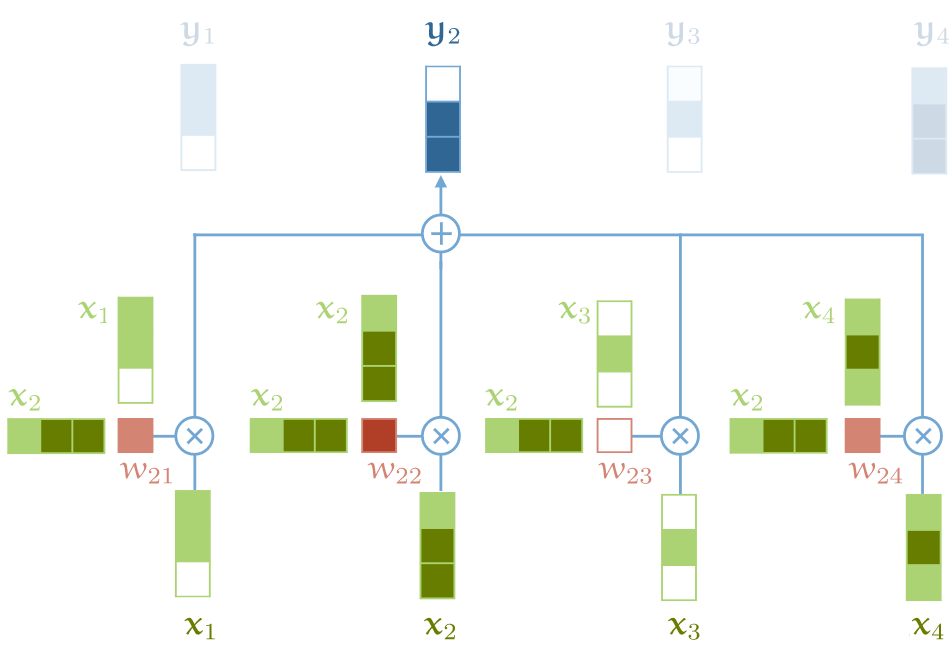
\includegraphics[width=\textwidth*3/4]{figs/self-attentoin-copied.PNG}
    \caption{Basic self-attention opertation illustrated. Example computation involved in calculating the output-vector $y_2$}
    \label{fig:basic-self-attention}
\end{figure}

Self-attention is the most important part of the Transformer architecture. In a nutshell, self-attention is a operation that transforms a sequence of vectors ($x_1, x_2, ... , x_t$) into another sequence of vectors ($y_1, y_2, ... , y_t$). And in order to calculate the output vector $y_i$ we take a weighted sum of the input sequence as follows: 
\[ y_i = \sum_j w_{ij} \cdot x_j \]
Here $j$ indexes the whole sequence, and the weights $w_{ij}$ aren't parameters but derived from a function of the input vectors $x_i$ \& $x_j$ 
\[ w'_{ij} = x_i^{\top} \cdot x_j \]
Moreover, finally, we take the softmax across each column (or j in this case) because we don't want the weights to explode and derail the model.
\[ w_{ij} = \frac{exp(w'_{ij})}{\sum_j exp(w'_{ij})} \]

\subsubsection{Understanding Self-Attention}
Suppose the problem of creating a recommendation system for books. One way to go about this is to go through the complicated and costly process of building features or vectors by hand. Let's say each dimension in the vectors represent a genre (like drama, romance or action) and for books, it defines how romantic or dramatic or action-heavy it is. For users, it defines how much drama or romance or action does the user like to read. Then for each pair of a book ($b_1, b_2...$) and user ($u_1, u_2...$), we can take the inner-product of the two vectors to obtain a score: 
\[ \text{score} = \sum_i b_i \cdot u_i \]
A high score tells us that the user will likely enjoy the book and a low score means they will most likely not enjoy the book. Intuitively, if a book has much romance, it will have a high component in the romance dimension and if a user also likes romance, they will also have a high component in the romance dimension. This means that two large numbers get multiplied together, increasing the score. On the other hand, if the user didn't like romance, they would have a low or possibly negative magnitude in that dimension and the product will thus reduce the score. Finally, if both the user and the book have a negative component for a dimension, the product will be positive and augment the score.

\subsubsection{Properties of Self-Attention}
Self-attention doesn't see its input as a sequence and instead views it as a set. This makes it parallelizable, which is a significant advantage when compared to Bahadanau Attention. Further, if we permute the input sequence, then the output is the same, just permuted with the same operation, which makes it \textit{permutation equivariant}. 



\subsection{Automatic Text Summarization}
\label{auto-text-summarization}
Automatic Text summarisation produces a concise and fluent summary while keeping the critical pieces of information and the overall message intact. This project aims to examine the effect of translation on summarisation and therefore. However, we will be concentrating on the Translator model more. We still need to build up an understanding of how automatic summarization is traditionally performed.

\subsubsection{Extractive Vs Abstractive}
 There are types of summarisation methods: Extractive and Abstractive. As the name suggests, Extractive Summarization aims to extract the text's critical information verbatim by employing various methods to rank phrases in the text and pick the ones it deems most important. Hence, it does not lead to very fluent summaries. On the other hand, Abstractive summarisation methods interpret and understand the text before generating the summary with the most crucial information. Although the summaries produced by abstractive methods output more readable summaries, they often lack essential information because they must deal with the complex problem of semantic correctness. 

\subsubsection{Bottom-Up Abstractive Summarization}
Interestingly, in the paper \cite{summary}, the authors came up with a revolutionary method to use extractive methods as a content selector to overproduce phrases and sentences from the text that should be incorporated into the summary. Then they used this content selector as Bottom-Up attention to restrict the abstractive step to the chosen key phrases, thus boosting the ability of the abstractive summarise to compress text while still retaining the ability to produce fluent summaries.

\subsection{Subwords}
\label{subwords}

\subsubsection{The necessity of Subwords}
All NLP tasks are trained on some fixed vocabulary, even though the problem they are trying to solve is almost always have an open vocabulary. This means that we will regularly come across out-of-vocabulary words when we are testing and evaluating the system. When it comes to translation models, they are expected to break compound words into their parts and translate them. One way to accomplish this is to use subwords. 

\subsubsection{Intuitive explanantion of why it works}\footnote{\red{Please let me know if this example is appropriate}}
For example \\
\begin{center}
    \changedFont{brushed} $\longrightarrow$ \changedFont{brush $+$ ed}
\end{center}
As described here, the verb \textit{"brush"} is modified to a past tense form with the addition of the \textit{"ed"} at the end. The model now only needs to learn how to translate \textit{"brush"} into the target language and then apply the modification for the tense, whereas, if we had tokenized by white space, the model would have to learn to translate both \textit{"brush"} and \textit{"brushed"}.

This improved ability to deal with rare and out-of-vocabulary words comes at the cost of computation owing to the fact that the sequence length increases. 

\subsection{Byte-Pair Encoding}
\label{bpe}
As described above, subword tokenization performs better than traditional tokenize-by-white-spaces. Byte-Pair Encoding is one method to perform subword tokenization and it is the method employed in this project. This algorithm has the same name and is based on the Loss-Less data compression algorithm. Once the entire text is loaded, the algorithm follows the steps: 
\begin{enumerate}
    \item Iteratively all character pairs are counted
    \item The most frequently occuring pair is concatenated to form one word
\end{enumerate}
These steps are repeated until the target vocabulary size is reached or the target number of merge operation is exhausted. 

\section{Project Management}
\label{project-management}


\subsection{Functional Requirements}\footnote{\red{The aim here is to list out the items implemented}}
\label{functional-requirements}

\begin{description}
    

\item[Corpus Preprocessing] The parallel corpora must be constructed. It is then tokenized with longer sentences dropped and divided into bins ready to form batches. The Translator model consumes these batches during training. 

\item[Transformer] The model implemented, trained and finally, deployed during the evaluation step. In order to achieve this, the architecture along with its sublayers must be understood to a high degree, especially the self-attention layer.  

\item[Training] The inherently parallel nature of Transformers requires the development of a training algorithm that can exploit this feature. Also, validate the model after each epoch. 

\item[Evaluation] Use the translator models of varying quality to translate the articles in the evaluation dataset (gv-snippet and gv-crowd) and then produce summaries. Finally, calculate the BLEU and ROUGE scores on the translation and summaries, respectively, searching for a correlation.  

\end{description}

\subsection{Non-Functional Requirements}
\label{non-functional-requirements}

\begin{description}
\item[Storage]
The datasets used and the translation models have a massive size. Therefore, any programs developed must make effective use of limited memory available on the Colab Notebooks. In a way, being economical with memory is more important than throughput.

\item[Efficiency]
The second most important consideration to take into account when building machine learning systems is efficiency or throughput. This pertains to developing programs that suit the computing architecture they run on (for example, GPUs) and minimizing any unnecessary computation. Thus, making intelligent use of the time available. 
\end{description}

\subsection{Tools Utilized}
\label{tools-utilized}

The rationale behind the language, libraries, Corpora and GPU-provider used in the project is discussed in this section. 

\subsubsection{Language}
The Programming Language adopted for the implementation of this project was chosen to be Python. It has become the standard language used for creating, training and deploying machine learning models. On top of this, it has many APIs for processing data, making it a better choice than another language like Java, which has machine learning libraries. 

\subsubsection{Libararies}
The main Python Libraries used in the project are: 
\\\\
\begin{description}
% {\textit{PyTorch \cite{torch}}} 
\item[PyTorch \cite{torch}]
The Machine Learning Library used to implement the Transformer architecture. It also provided implementation for the Embedding, Linear, Layer Normalization and Dropout used to create the Transformer. 
% {\textit{SentencePiece\cite{sentencepiece}}} 
\item[Sentence-Piece \cite{sentencepiece}]
In a pre-processing step, it was used for tokenization. It is an unsupervised and language agnostic text tokenizer and detokenizer. It is used in NLP whenever the vocabulary size is already established. Most importantly, they are vital in building end-to-end systems such as the translation-then-summarize models being tackled in this project.  
% {\textit{openNMT-py}} 
\item[OpenNMT-py]
A generic deep learning framework specialized in sequence-to-sequence model. It provided and deployed the pre-trained summarization model.
% {\textit{SacreBLEU\cite{sacrebleu}}} 
\item[SacreBLEU \cite{sacrebleu}]
A standard implementation of BLEU \cite{bleu} which takes the detokenized output and reports shareable and comparable BLEU scores. 
% {\textit{ROUGE}} 
\item[ROUGE]
A Python API that reports the ROUGE metric (from the paper\cite{rouge}). 

\end{description}

\subsubsection{External Software}
The external software employed in development and security for the project are listed here:
\begin{description}
% {\textit{PyCharm}}
\item[PyCharm]
An IDE for python integrated with Git was used for programming and version control and environment management. 

% {\textit{Jupyter Notebook}}
\item[Jupyter Notebook]
It is a web application that aids in creating and sharing documents containing code, visuals, and equations. Colab Notebooks, which are used to run the project, are Jupyter Notebooks hosted on Google's server with access to GPUs. 

% {\textit{Git}}
\item[Git]
A version control software used to backup code to keep it safe along with versioning as well. 

% {\textit{Google Drive}}
\item[Google Drive]
The datasets used, the models' features and the output generated was stored on Google Drive, easily accessible to the Colab Notebooks. 

% {\textit{Overleaf}}
\item[OverLeaf]
\red{should I mention?}

\end{description}


\subsubsection{Dataset-Training}
For training the translation models, the News-Commentary\footnote{https://opus.nlpl.eu/News-Commentary-v11.php} parallel corpora (with about 200K sentence pairs) and a portion of the ParaCrawl\footnote{https://opus.nlpl.eu/ParaCrawl.php} parallel corpora (with about 30M sentence pairs) were used. 

\subsubsection{Dataset-Evaluation}
For evaluation, the global-voices datasets (from the paper \cite{nguyen-daume-iii-2019-global}) were used. It has the hand translated articles in markdown files and, most importantly, two JSON objects (gv-crowd and gv-snippet) with the summary and a list of languages the article is present in along with their filenames. The summaries associated with each JSON: \begin{itemize}
    \item gv-crowd: contains the handwritten summaries obtained by crowdsourcing the summaries also referred to as the gold standard in NLP. 
    \item gv-snippet: contains the summary from the Global Voices website, the first 50 words in the article.
\end{itemize}

\subsubsection{GPU}
Translation models using the Transformer architecture are massive, a size larger than 200MB. Therefore, the models were trained on a Cloud Computing Cluster with access to GPUs like the HPC in Cambridge. Nevertheless, the long wait times caused a switch to operate the training procedure on Google-Colab, where one can connect the Colab-notebook to Google's Nvidia K80 GPUs for free but only 12 hours at a time.



\subsection{Software Engineering Approach}
\label{professional-approach}

In this project, I have tried my best to follow the Software Engineering Process, which starts with understanding the core requirements and investigating their feasibility to figure out the restrictions. Followed by designing a solution, however, this was already covered in the papers \cite{transformers} for the translator model architecture and the paper \cite{nguyen-daume-iii-2019-global} for the evaluation methodology, and finally, programming, training \& testing the model.  
\\\\
The code was developed and tested first on a 64 bit Windows 10 (Home) laptop and then on Google Colab's notebooks. Code was periodically backed up to Google Drive and a secondary Hard Disk to protect against corruption or failures. The GitHub repository was updated every day. Any changes can be quickly applied to the notebooks where the programs were running, allowing for quick and easy code portability. 



%%%%%%%%%%%%%%%%%%%%%%%%%%%%%%%%%%%%%%%%%%%%%%%%%%%%%%%%%%%%%%%%%%%%%%%%%%%%%%%%%%%%%%%%%%%%%%%%%%%%%%%%%%%%%%
%%%%%%%%%%%%%%%%%%%%%%%%%%%%%%%%%%%%%%%%%%%%%%%%%%%%%%%%%%%%%%%%%%%%%%%%%%%%%%%%%%%%
\chapter{Implementation}
\label{implementation}

\section{Pre-processing}
\label{pre-processing}
This section describes the steps followed in processing the datasets to mould them into a compatible form with the Transformer implementation. These are very general and can be applied to any large dataset. 

\subsection{Dataset Clipping}
\label{dataset-clipping}
The datasets that are being used for this project are ParaCrawl(v5) and News Commentary(v11)\footnote{Links to the datasets can be found in section \ref{tools-utilized} \nameref{tools-utilized}}. The data is provided in the form of two raw text files, one for each source/target language. One sentence per line and the $n^{th}$ sentence in each file are translations of each other. Because of the computational resources and the time available, it was decided that less than 1 million pairs of sentences in the source (fr, es, de) and target (en) language will be used in the training step. However, ParaCrawl and News Commentary combined have over 30 million sentence pairs and is, therefore, too large to handle. Therefore, a dataset containing sentence pairs from News Commentary (200K) and ParaCrawl (top 800K) was constructed. Since the final evaluation was meant to be on the gv-crowd/gv-snippet dataset from the paper \cite{nguyen-daume-iii-2019-global} which is mostly news articles and their translation and summaries, the News-Commentary dataset was used. However, the News-Commentary dataset was too small to train the models properly; thus, another 800K sentence pairs were taken from the ParaCrawl dataset. Considering the large size of the datasets, it was essential to build a memory-efficient program to accomplish this. 



\subsection{Tokenization}
\label{tokenization}

\subsubsection{Vocabulary Size}
Important considerations that need to be taken when tokenizing with BPE is the vocabulary size. During the execution, it came to light that a larger vocabulary size brings the mean sequence length down. Shorter sequences mean that the computational complexity will be reduced. 

\begin{figure}
    \centering
    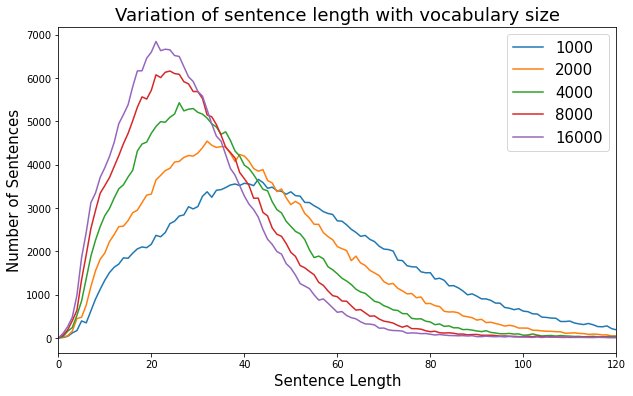
\includegraphics[width=\textwidth*3/4]{figs/length-vs-vocab-size.png}
    \caption{Graph showing the distribution of sequence lengths with different BPE vocabulary sizes. There is clear shift towards having more short seqeunces and shorter seqeunces than before.}
    \label{fig:sentence-length-vs-vocab-size}
\end{figure}
Upon further investigation, it was concluded that because BPE is a greedy algorithm and if the vocabulary size is large, it will assign one subword to the most frequently occurring words. As a result, reduce the average length of the sequences. Regardless of the computation boost, it undoes most of the benefits described above. After reaching this conclusion and with the help of the analysis conducted in the paper \cite{vocabsize}, the vocabulary size was set to \textbf{8000}.
\subsubsection{Sentence Piece}

It provides many functions for subword tokenization like the one being used for this project, BPE. A benefit of using Sentence Piece is that it takes raw files as its input. Consequently, to learn the vocabulary model, the previously generated dataset with a million sentence pairs is used in their raw text file format along with: 
\begin{itemize}
    \item \lstinline{model_type}: to specify 'BPE'
    \item \lstinline{model_prefix}: to specify the name of the model. Use later in the pipeline
    \item \lstinline{vocab_size}: set to 8000
    \item \lstinline{character_coverage}: set to 1.0 to specify complete character coverage. 
    \item \lstinline{pad_id}: set to 3 since the default(-1) causes problems further down the pipeline. 
    
\end{itemize}
The Sentence Piece model only needs to train once. Whenever it is needed to tokenize or detokenize, it just needs to be loaded into our program by using the \lstinline{model_prefix}. 

\subsubsection{Truncation}
Once the vocabulary model has been used to tokenize the sentence into a sequence of IDs (the indices in the vocab dictionary), the sequence's size needs to be checked. It is impossible to train on very long sentences because the computation graph computed during the backpropagation is so huge that it leads to an Out-Of-Memory (OOM) Exception. 

As a result, a maximum length restriction was added. Thus, introducing another hyperparameter that must be set to an appropriate value; else, it can completely wreck the training process. In the article \cite{training-tips}, the authors examined and reported the following graph: 

\begin{figure}
    \centering
    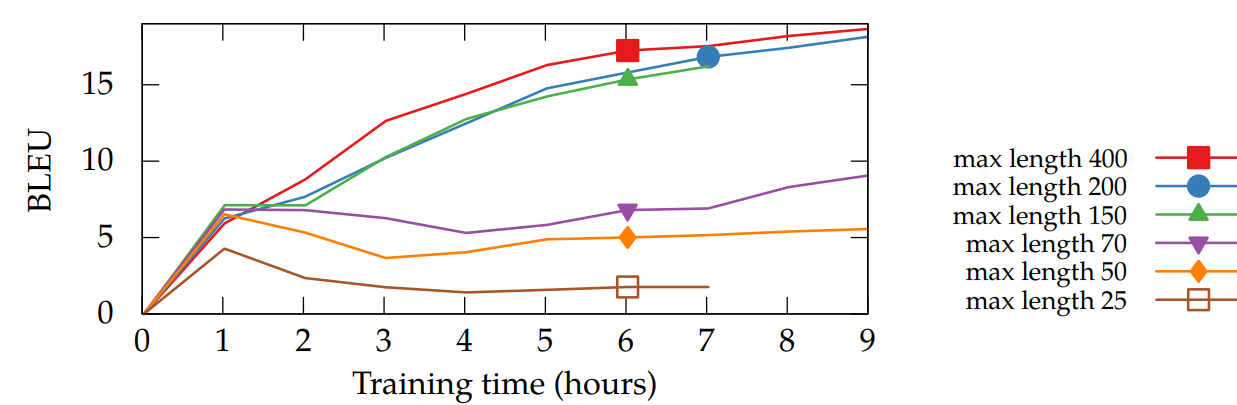
\includegraphics[width=\textwidth]{figs/fig4frompaper-trainingtips.PNG}
    \caption{The effect of various maximum length values performed. Taken from the paper \cite{training-tips}. It presents that setting max length to a small value like 25, 50 or 70 will hinder performance on the test corpra.}
    \label{fig:figure-4-from-paper}
\end{figure}

It is suggested that the lowest possible maximum length should be used. This is essentially a trade-off between the complexity arising from the extensive computation graph calculation and generalizability.
Something from the \textit{Deep Neural Networks (Unit of Assessment)} which is quite pertinent here is that all sequence models do not generalize to longer sequences if they were exposed to only short sequences during the training process.

\subsubsection{Applying padding}
After tokenization and removing the long sentences, padding needs to be added to the sequences to make them the appropriate length. The length is decided by the structure of the \textbf{bins} described below. It also ensures that the source/target sequence have the same number of tokens. The sequences need to be the same size because it helps calculate the overall tokensize of each sentence pair, which aids in calculating batch sizes. Moreover,  in a PyTorch Tensor, the size of each sequence in a batch should be the same; else, it leads to an Error. Therefore, keeping both the source/target sequences the same length aids in decreasing the complexity of the batching algorithm though at the cost of efficiency. 

\subsection{Bins}
\label{bins}
This section details a method adopted to increase efficiency by altering the scheme in which padding tokens are added to the sequences. When we pass a sequence to the Transformer, an equal amount of computation is performed on the actual tokens and the padding tokens. 

Consider a na\"ive approach where all the sequences are padded to be maximum length. It will require a basic batching algorithm that can assign any sequence to a batch. However, considering the above argument, a large portion of the computation will be wasted. In other words, to increase the throughput of the Transformer in training, the number of padding tokens in each sequence should be minimized.  

Keeping this in mind, the first approach was to use bins of some fixed size like \\$\text{bins} = [32, 40, 48, 56, 64...152]$. In this method, each pair is assigned to the bin corresponding to $b$ size, provided the source and the target sequence length is less than or equal to $b$, where $b \in \text{bins}$. The two sequences then have padding tokens added to them so that their size equals $b$. 

Considering how well the first approach faired against the initial na\"ive approach, the next and final approach was to use bins of width one and reduce the minimum size of the bins since examination revealed there were tons of shorter sequences in French, i.e. $\text{bins} = [10, 11, ... \text{max length}]$. As shown in the graph in Figure \ref{fig:distribution-across-languages}, French peaks at around 20 to a value of 70K sentences. 
\\\\

\begin{figure}
    \centering
    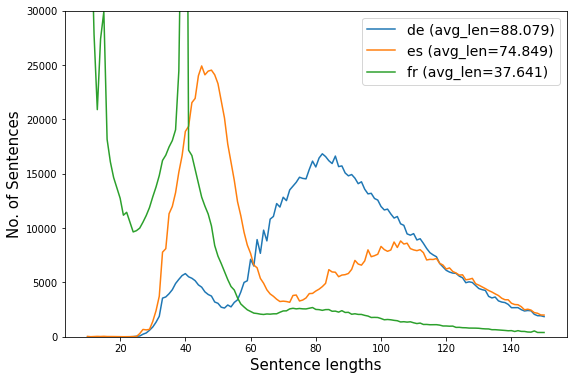
\includegraphics[width=\textwidth*3/4]{figs/length-distribution-across-languages.png}
    \caption{Graph shows the distribution of sentence lengths across the 3 languages used. The sentences lengths chosen for each sentence pair was the maximum of the source/target sequence after tokenization with BPE(vocabulary size 8000).}
    \label{fig:distribution-across-languages}
\end{figure}
    

% Please add the following required packages to your document preamble:
% \usepackage{multirow}
\begin{table}[]
\centering
\begin{tabular}{ccccc}
\toprule
\multirow{2}{*}{Tokensize} & \multirow{2}{*}{Raw} & \multicolumn{3}{c}{Effective} \\
\cmidrule(l){3-5}
                           &                      & naive    & big      & small  \\
                           \midrule \midrule
1024                       & 15.9k                & \textbf{4.7k}     & 14.9k    & 16.7k   \\
2048                       & 15.5k                & 4.3k     & 14.4k    & 19.4k   \\
3072                       & 16.4k                & 4.5k     & 15k    & 24.6k   \\
4096                       & \textbf{16.6k}                 & 4.3k     & \textbf{15.5k}    & \textbf{30.0k}  \\
\bottomrule
\end{tabular}
\caption{The Raw and Effective training throughput for different tokensizes and batching methodologies that were discussed above. It was also found that 30\% of tokens in each batch for the Na\"ive approach were actual tokens (not pads). Similary for Big and Small approach it was 91.8\% and 99.8\% respectively}
\label{table:raw-and-effective-throughpu}
\end{table}

% random batches of some average length 


\section{Transformer Architecture}
\label{transformer-architecture}

For this project, the Transformer(\textit{Base}) architecture was used. It is smaller and does not perform as well as the Transformer(\textit{Big}) architecture, but it is much smaller and meets our computational restrictions. In this section, various parts of the architecture are discussed and how they were implemented in PyTorch. 

\begin{figure}
    \centering
    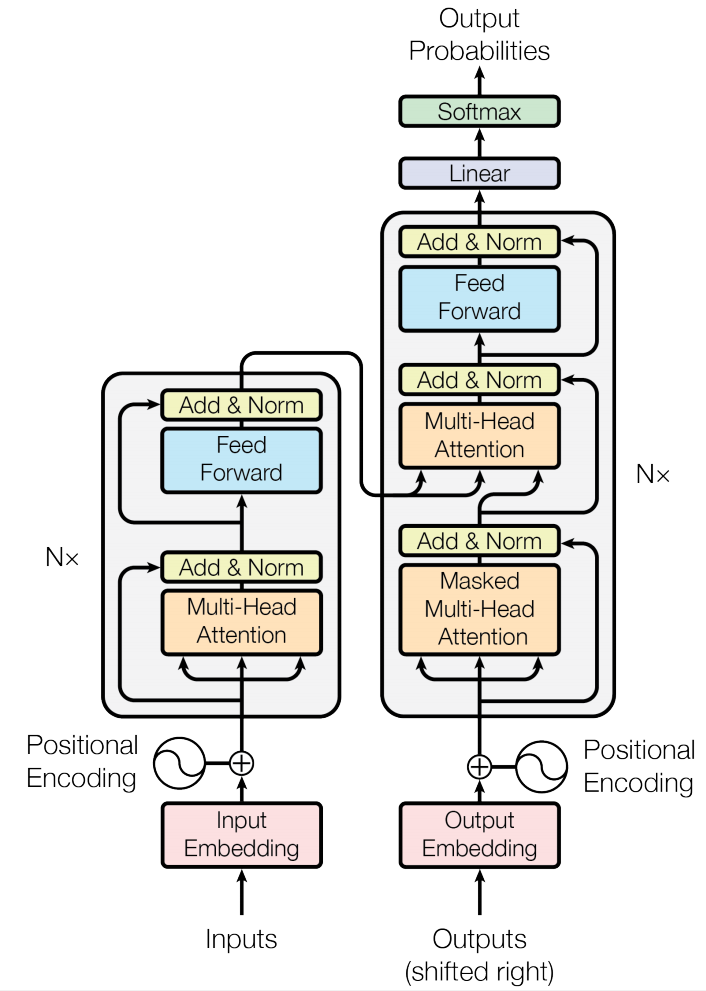
\includegraphics[width=\textwidth/2]{figs/transformer-architecture.PNG}
    \caption{The Transformer architecture from the paper \cite{transformers}}
    \label{fig:transformer-architecture}
\end{figure}

\subsection{Embedding layers}
\label{embedding-layers}

A batch of sequences is passed to the Transformer in the form of a matrix with the shape [B x S], where B is the number of sequences in the batch and S is the sequence length. The words are one dimensional token IDs and need to be converted to embedded vectors with a size equal to the model dimension ($d_{model} = 512$ for \textit{base}). \lstinline{torch.nn.Embeddings} was used to implement this layer which learns the embeddings for each token. The Embedding Layer is an integral part of the Transformer because the embedded vectors are critical to the attention sublayers, which learn to exploit the embeddings to understand the relationships between words in the sequence. 

\subsection{Positional Encoding}
\label{pe}
Each operation in this architecture is either point-wise (like embedding or feed-forward) or view the sequence as a set (like attention or linear norm). Therefore, the model does not know the relative or absolute position of the token in a sequence.  Out of the many ways to overcome this issue, the authors in \cite{transformers} suggested using sine and cosine functions with the wavelength in a geometric progression commencing at $2\pi$ to $10000 \cdot 2\pi$. These are formulated as follows: 
\begin{align*}
    PE_{p, 2i} &= sin(p / 10000 ^ {(2i/d_{model})})\\
    PE_{p, 2i+1} &= cos(p / 10000 ^ {(2i/d_{model})})
\end{align*}
where $p$ is the position of the token in the sequence and $i$ is the dimension. These Positional Embeddings (PE) are injected 

During implementation with PyTorch, it was crucial to turn the matrix with 150 x 512 items into a PyTorch buffer. Doing so allows PyTorch to track and store the PE as parameters. They move between the CPU and GPU like the features, but they are not part of the Statistical Gradient Descent (SGD).

\subsection{{Atttention}}
\label{attention}

What is described in the section \ref{background} \nameref{background} is the basic version of Self-Attention. This operation has been enhanced with three keys advances. These are using Query, Key and Value matrices, scaling the dot product, Multi-head attention.

\subsubsection{Queries, Keys \& Values}

Every input vectors $x_i$ is utilised in 3 different ways in the self-attention operation:
\begin{itemize}
	\item \textbf{Query}:  it is utilized to calculate the weights for its output vector $y_i$
	\item \textbf{Key}:  it is utilized to calculate the weights of all the output vectors $y_j$
	\item \textbf{Value}:  it is included in the final weighted sum to get the output vectors after the weights have been ascertained. 
\end{itemize}

In the basic version, we utilise the input vectors for all these three roles of Query, Key and Value. While in this version, learnable parameters are injected in the form of matrices $W_q$, $W_k$ and $W_v$ to build separate vectors for each role which can help form better output vectors. These matrices are built using \\ \lstinline{torch.nn.Linear} (which are fully connected neural networks)

\begin{align*}
    q_i = W_q x_i \qquad       k_i & = W_k x_i \qquad     v_i = W_v x_i \\
    w'_{ij} & = q_i^\top k_j \\
    w_{ij} & = \text{softmax}(w'_{ij}) \\
    y_i & = \sum_j w_{ij} v_j
\end{align*}

\begin{figure}
    \centering
    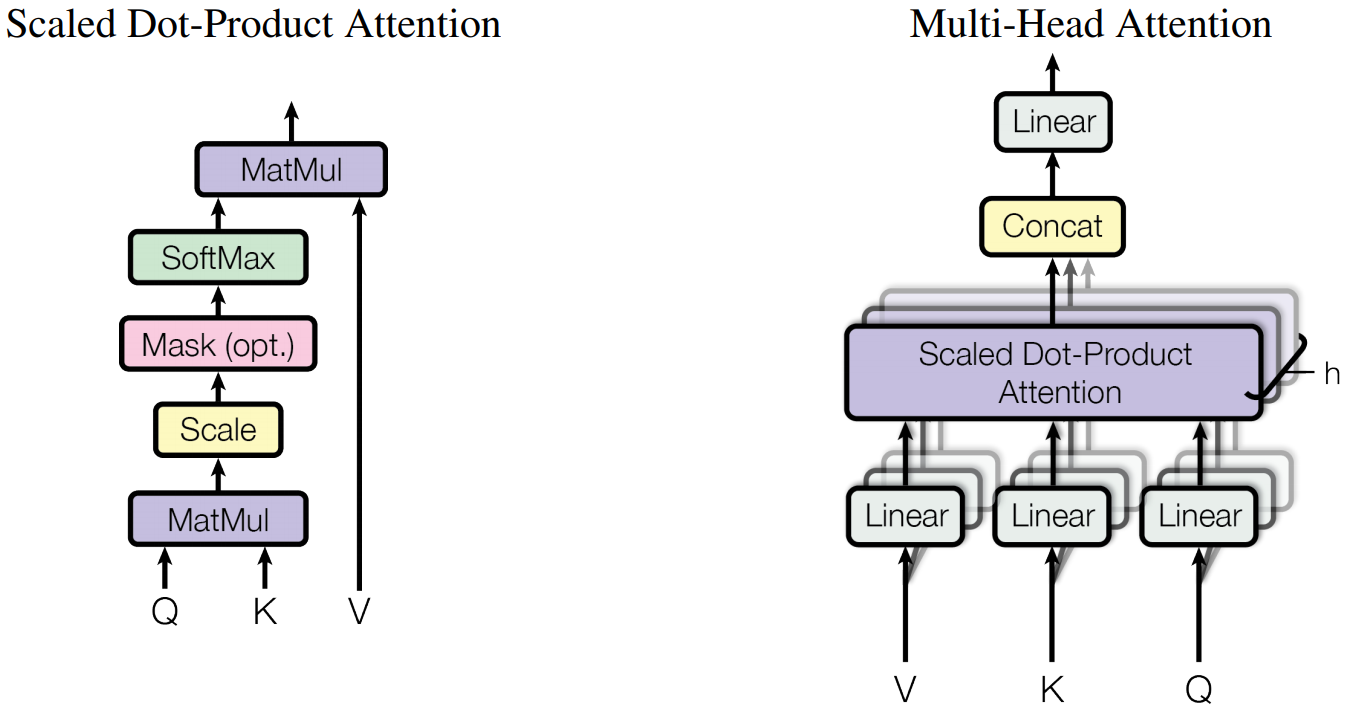
\includegraphics[width=\textwidth]{figs/multihead-attention.PNG}
    \caption{Displaying the Scaled Dot Product (left) and Multi-head Attention mechanism (right) with multiple attention layer running in parallel. Taken from the paper \cite{transformers}}
    \label{fig:my_label}
\end{figure}

\subsubsection{Scaled-Dot product}

Since there is a softmax operation involved, the large values that appear may completely ruin the results after this operation and cause the learning to come to a complete halt. 
Therefore, the scaling factor that is decided to be $1/\sqrt{d_k}$.
Where the size of the Query and Key vectors are $d_k$ and the size of the Value vectors is $d_v$

\[ w'_{ij} = \frac{q_i^\top k_j}{\sqrt{d_k}} \]

\subsubsection{Multi-head Attention}

The current implementation can, over time, learn to pick up on how each word in the sequence is related to another. It is obvious that all of these relationships get summed into one and arguably makes it more complex and, therefore, more troublesome to learn. For example, in the sentence: 
\begin{center}
    \changedFont{ "Ana took chocolates from Bob"} 
\end{center}
Here \textit{"took"} is related to "Ana", "Bob" and "chocolates". Albeit in entirely different ways as \textit{Ana} is someone who takes; \textit{chocolate} is the something that is taken and finally, \textit{Bob} is the one who gives. This is just one of the complex relationships that need to be learnt and very hard with a single self-attention operation. 
\\\\
A simple solution is to use multiple self-attention operations (instead of just one) and combine the results. These are called \textbf{attention heads} and indexed them by $(\cdot^r)$. Consequently, $W_q$, $W_k$ and $W_v$ turn into $W^r_q$, $W^r_k$ and $W^r_v$

\subsubsection{Narrow or Wide Multi-Head Attention}

There are two ways to implement the Multi-head Attention mechanism. These are the Narrow and Wide approaches. To explain it further, suppose our input vectors with the dimensionality of 512 as before and the number of attention heads we are using is 8. 

In the Narrow Multi-head attention approach, our matrices $W^r_q$, $W^r_k$ and $W^r_v$ will have the size 512 x 64 and at the end, we will be simply concatenating the output from each head to get back to the size of 512. 

While we are following the Wide Multi-head Attention approach, the matrices will be 512 x 512 and at the end, we will have to use a Neural Net to condense from a size 4096 to 512.

\subsubsection{Current Implementation}
The Narrow Multi-head attention approach was applied in this project. Accordingly, the Query, Key and Value matrices were built as \lstinline{torch.nn.Linear} layers with input and output size set to the same value ($d_{model}$. After the query, key and value vectors are calculated, they are transformed from a size of [B x S x D] to [B x S x H x d], where B and S are as defined before; H is the number of heads; D is the $d_{model}$ and d (=D/H). Then we follow the self-attention methodology as described before. 

\subsection{Position-Wise Feed Forward Netowrks}
\label{fc2}
After the attention layers, both the Encoder and decoder contain a two-layer point-wise Feed-Foward network which performs a linear transformation with a ReLU (Rectified Linear) activation in between them and an inner-layer dimensionality of $d_ff=2048$. 

A single layer point-wise feed-forward Network is used at the end and applied to the decoder's output. It takes the decoder's output and transforms the vectors from $d_{model}$ to vocabulary size, from 512 to 8000. Lastly, we apply a softmax layer and this gives us the output probabilities for each word at each index. 

\subsection{Regularization}
\label{regularization}
There are two regularisation methods applied: Residual links and dropout. 

\subsubsection{Dropout}
Dropout is ignoring some randomly chosen nodes. It is used during training for deep models to ensure that the model does not overfit the training set. It also ensures that the model generalises better to unseen data. The dropout rate was set to 0.1 

\subsubsection{Residual Connections}
Residual connections are adding the input of a sublayer to the output from the sublayer: 
\[ y = x + \text{SubLayer}(x)\]
Unlike traditional models, the data path through residual networks varies in length and allows the model to work as an ensemble of networks. Non-linear activations naturally cause the gradients to explode or vanish for very deep networks. The addition of these 'skip connections' allows the gradient to flow through directly and undercut the non-linear activations' problem. 

\subsection{Layer Normaliation}
\label{layer-norm}
Between each sublayer (multi-head attention and feed-forward) layer normalisation is carried out. The layer normalisation ensures that there is a smoother gradient, faster training and allows for better generalisation. 
Layer normalisation is vital; however, when it is carried out is equally relevant, i.e. after (Eq \ref{eq:norm-after}) or  before (Eq \ref{eq:norm-before}) every sublayer. A significant problem during the training process was that the model developed with the normalise-after methodology would not converge at all. After spending hours experimenting with each of the model's components extensively, the solution was found thanks to the explanations in the paper \cite{layernorm}. The authors advised using the normalise-before method because it diminishes the dependence of the output on the residual branches. However, they did criticise the normalise-before method as it did not produce models of the same quality as normalise-after. Considering this trade-off, the normalise-before methodology was selected. 

\begin{equation}
    y = LN(x + \text{SubLayer}(x))
    \label{eq:norm-after}
\end{equation}

\begin{equation}
    y = LN(x) + \text{SubLayer}(LN(x))
    \label{eq:norm-before}
\end{equation}

\subsection{Encoder and Decoder}
\label{enc-dec}

The Encoder/Decoder in the Transformer is built using multiple identical layers, further elaborated upon below. The output from each Encoder/Decoder layer is passed directly to the next with the same masks. 

\subsubsection{Encoder Layer}
Each Encoder layer comprises two main sublayers, the multi-head attention and the point-wise feed-forward operation with a layer normalisation before each layer and residual connections across each sublayer. 

\subsubsection{Decoder Layer}
Each decoder comprises three main sublayers the multi-head attention layer, point-wise feed-forward layer and an encoder-decoder attention layer. The encoder-decoder attention layer is a multi-head attention layer with the Keys and the Queries set to the Encoder's output. 


\section{Training}
\label{training}

\subsection{Hyperparameters}
\label{hyperparameters}

This subsection discusses the hyperparameters and why the values were chosen. 
\\\\
\textbf{Dataset size}: A larger dataset size has been shown to improve the translation model's quality. However, as discussed in section \ref{dataset-clipping}, this was set to one million sentence pairs because of the time and memory restrictions.  
\\\\
As discussed in the subsection \ref{tokenization}:\\
\textbf{Vocabulary size} was chosen to be 8000.
\\
\textbf{maximum length} was chosen to be 150.
\\\\
\textbf{Layer Normalization} was set to before each sublayer within the encoder/decoder units, as discussed in the subsection \ref{layer-norm}.
\\\\
\textbf{Batchsize} for a transformer is often referred to as tokensize. Tokensize is defined to be the product of the number of sequences and the length of the sequence. In the first assignment \textit{Deep Neural Networks Unit of Assessment} an experiment on the effect of different batch sizes and learning rates was conducted. It shed light on the fact that having a larger batch size leads to faster convergence, provided that the learning rate is reasonably low. Similar conclusions were reached in the paper \cite{training-tips}, which showed that having a larger batch size raises not only the throughput but also improves the BLEU score, albeit to an extent. Nevertheless, the maximum number of tokens used on Google Colab's GPU was limited because of the memory restrictions and was approximately 7500. 

After weighing all of these findings, the batch size/tokensize was set to $4096$. A power of two was used, keeping in mind the GPUs' architecture, which tends to have some power of 2 execution units. Hence, when work gets scheduled, we will not have too many execution units sitting idle and thus, improve the throughput. 
\\\\
\textbf{Optimizer hyperparameters} following the implementation from the paper \cite{transformers}, the Adam optimizer \cite{adam}, with $\beta_1 = 0.9$; $\beta_2=0.98$ \& $\epsilon=10^{-9}$. The learning rate was first increased linearly for the \textit{warmup\_steps} and then decreased proportially to inverse square-root of the number of steps: 
\[ lr = d_{model}^{-0.5} \cdot min (\text{step\_num}^{-0.5}, \text{step\_num} \cdot \text{warmup\_steps}^{-1.5}) \]
The choice of \textit{warmup\_steps} was taken from the paper \cite{training-tips}, which concluded that using less than 12k \textit{warmup\_steps} can lead to divergent training. Consequently, it was set to \textbf{16k}. 
\\\\
The rest of the hyperparamters were chosen according to the \textit{BASE} architecture in the paper \cite{transformers}. \\
\textbf{Model Dimensions} was set to \textbf{512}
\\
\textbf{number of attention heads} was set to \textbf{8}
\\
\textbf{number of encoder-decoder layers} was set to \textbf{6} each
\\
\textbf{dropout} was set to \textbf{0.1}
\\
Finally, out of the two Narrow and Wide multi-head attention, described in the subsection \ref{attention}, the \textbf{Narrow} version was implemented. 


\subsection{Training step}
\label{training-step}
\subsubsection{Batching}
\begin{figure}
    \centering
    \begin{lstlisting}
    def batch(bins: Dict[int, List[List[int]]], tokensize: int):
        
        
        
    \end{lstlisting}
    \caption{Batching algorithm \red{should I include this?}}
    \label{fig:batching algorithm}
\end{figure} The batching algorithm is implemented as a generator\footnote{Generator Functions allows to declare the function that behaves like an iterator, i.e. it can be used in a for loop} function in python in order to simplify the code. It begins by shuffling the order of the sentence pairs in each bin. It then chooses a random bin and builds a batch by selecting the required number of sequences from the bin. \\
Thus batch iterator returns two 2d arrays of the shape [$tokensize // b$, $b$], one each for the sequence in the source and target languages. \\
Where the bin size is $b$ and the tokensize/batch size is $tokensize$, then the required number of sequences is the output of the integer division of the two: $tokensize//b$. 



\subsubsection{Inputs and Outputs}
The 2d-arrays from the batch iterator need to be transformed into a compatible form with the training step. The source array gets converted into a \lstinline{torch.LongTensor} and is moved onto the GPU. 

\begin{lstlisting}
    target_tensor_input = target_array[:, :-1]
    target_tensor_output = target_array[:, 1:]
\end{lstlisting}

 For the target array, first a beginning-of-sequence of character \lstinline{<bos>} \& a end-of-sequence character \lstinline{<eos>} is added at the appropriate position. The above code represents the transformations carried out on the target array.
Then for each sequence in the batch, all but the last item is used to build the target tensor. 
The expected output from the Transformer is set to a \lstinline{torch.LongTensor} constructed from the target array with every item in each sequence except for the first one.  

Consequently, the training algorithm is designed. For every position in the input target tensor, we expect to see the following word in the sequence to have the highest probability in the target predictions. The benefits of the immense \red{parallel-ability} of Transformers shines. Usually, the sequence models' with recurrent architecture require that the sequence is passed serially at both the encoding and decoding during the training step. However, with Transformers, the entire sequence moves through the model parallelly. 

\subsubsection{Masks}
Two types of masks need to employed to ensure that the attention operation works as expected. 

Firstly, perhaps the most obvious one, that is the \textbf{padding mask}. Pads were added to the source and target sequence to ensure they were the same length. These pads would be considered as part of the sequence if they were removed using masks. To build the padding mask for the sequences, the following code is used. 
\begin{lstlisting}[label=padding-code]
    padding_mask = (sequence != pad)
\end{lstlisting}

Another mask required is the \textbf{no peak mask} that will ensure that the decoder can't peak at the following (future) words when making it's predictions. To construct it the following code is used:
\begin{lstlisting}[label=nopeak-mask-code,caption=No Peak Mask generator]
def nopeak_mask(size):
    np_mask = np.triu(np.ones((1, size, size)), k=1)
    np_mask =  torch.from_numpy(np_mask) == 0
    return np_mask
    
# output for size=3
# [[[1., 0., 0.],
#  [1., 1., 0.],
#  [1., 1., 1.]]]
\end{lstlisting}

Here, an upper triangular matrix is constructed and then 1s and 0s get flipped to produce a matrix, as shown above. This nopeak mask is combined with the padding mask discussed before to form the mask for the target tensor. 

\subsubsection{Application}
In order to apply the mask, before the softmax operation, $-10^9$(a large negative number) is added to all those positions where the mask is 0. During the softmax operation, the element-wise exponentiation causes these values to be suppressed to zero. 

\subsection{Text Generation}
\label{text-generation}
Once a model has been trained. It will need to generate text. 
In an ideal world, we would search all possible sequences before returning the sequence with the highest probability. Nevertheless, resource restrictions mean that we have to settle for heuristic-based search algorithms for text generation like Beam Search or Greedy search.

The structure of any text generation algorithm is to generate words in steps, i.e. one at a time. With Transformers, first, the encoder output is calculated by passing the source sequence through the transformer-encoder as we did in training. The encoder output is used as the context/memory to inform the next generation and is passed to the transformer-decoder. At the start, only the beginning-of-sequence word \lstinline{<bos>} is passed to the decoder. As words are generated, all of them are used to inform the next word to be generated. Recognizing that the predictions will be a probability distribution on the entire vocabulary at each step, consider two implementations of text generation algorithms attempted in the project. 

\subsubsection{Greedy Search}
To understand how Beam Search works, it helps to look at a Greedy algorithm which is essentially a Beam search with a width of 1. Moreover, it is an easy to execute and quick algorithm that was used initially to evaluate/test the model before moving onto Beam Search. In this algorithm, the most likely word, i.e. the word with the highest value after the final softmax operation, is chosen as the predicted word. 

It is trivially straightforward why this algorithm does not do too well. Since the word probabilities might not be accurate initially, the first few words generated may be incorrect. This form of error piles up at each step as we move through the sequence. 

\subsubsection{Beam Search}
Beam Search is a pruned version breadth-first-search. There is some preset search width commonly referred to as $k$. The most significant difference from the Greedy Search is that we hold the top-k most likely words for each step. Hence, there is only one sequence at the start, and after considering 8000 words (vocabulary size), $k$ words are chosen, which form the $k$ sequences we will consider for the next word. In the next step and all subsequent steps, $k$ sequences are used to generate $8000 \cdot k$ words from which again $k$ words are chosen. The commonly used $k$ is about 5 to 10, and for the evaluation and translation steps, $k$ was set to 10. \red{should I incluce pseudo code}


\subsection{Model Evaluation}
\label{model-evaluation}
After each epoch\footnote{refer to section \ref{background}}, the model is evaluated by testing it on a small dataset comprised of the test sets in past WMT translation tasks. The test set had about 2000-3000 sentence pairs. For each sequence, the model produces a translation using the Beam Seach/Greedy Search described above in the subsection \ref{text-generation}. 

Following the translation, the BLEU scores were calculated (using SacreBLEU) and stored. For the first three epochs, the scores are just stored. Following that, for every subsequent epoch, the new BLEU score is compared to the average of the last three, and if there is no substantial improvement in the scores, then the training is stopped. A substantial difference here refers to an increase of $\leq 0.01$, i.e. the difference between the new score and the moving average must be $> 0.01$. 

\red{mention which ones exactly}

\section{Pipeline Overview}
\label{pipeline-overview}
This section reports all the work involved in the pre-processing, translation, summarization and post-processing involved in the final evaluation step. 

\subsection{Pre-Processing}
\label{preprocessing}
The following steps were followed to collect all the relevant data before moving onto the translation and summarization. 
\begin{enumerate}
    \item Load the JSON files (GV-snippet and GV-crowd)\footnote{refer to subsection \ref{requirements}}.
    \item Filter both the JSON objects so that they only contain the entries comprising articles in the required source language (de/es/fr). 
    \item Join the JSON objects into one. Here, the auxiliary information in both JSONs was found to be the same and thus, the snippet summary was copied into the current filtered GV-crowd JSON and under a new key. 
    \item The final step involved reading the articles in both the source and target language, provided as markdown files.
\end{enumerate}

\subsubsection{Processing the markdown article}
The markdown articles for all languages were such that there were two newline characters between each of the sentence. Hence, reducing the amount of processing needed to get down to the sentence level partition. Moreover, the English articles were quite clean. Whereas, the articles in French (fr), Spanish (es) and German (de), there were hyperlinks and, most importantly, extra text like \\
\changedFont{"Compártelo: Twitter Facebook Reddit google plus"}\\
Which in Spanish means: \\
\changedFont{"Share on Twitter Facebook Reddit google plus"}\\
These had to be cleaned before being fed the source articles into the translator. French and German had similar problems, but they were not as frequent, and therefore, nothing was done for them. 

\subsection{Translation}
\label{translation}
Using Beam Search described above in the subsection \ref{text-generation}, each sentence in the source language is translated into the target language (English). The translated sentences are then collected into one line and written to a file, and ready to be summarized. 

\subsection{Summarization}
\label{summarization}
As described in the \ref{auto-text-summarization}, the pre-trained summarizer following the Bottom-Up Abstractive architecture is used. Another benefit of using Jupiter notebook comes to light in this step: invoking shell commands within a for-loop in python and using python variables within the shell command. The hyperparameters used for the generation are as follows: 
\red{describe these penalties in the background section}
\begin{itemize}
    \item minimum length: 35
    \item Penalties applied were: Stepwise penalty, Coverage penalty (summary) and Length penalty (wu). 
    \item beam size of 20
    \item beta set to 5 and alpha set to 0.9
\end{itemize}

\subsection{Post Processing}
\label{postprocessing}

\red{needs work}\\
The evaluation's final step is to collect the hand-translated sentences and the machine-translated sentences together to calculate the BLEU score. After reporting the BLEU score, the predictions are collected together, and the mean rouge scores are reported in the \textbf{Chapter \ref{evaluation} \nameref{evaluation}} (specifically \ref{evaluation-results}). 


\section{Repository Overview}
\red{TODO: Need to wrap up the code and discuss the repo structure and choices involved.}


\chapter{Evaluation}
\label{evaluation}

\section{Evaluation Methods}
\label{evaluation-methods}

\subsection{BLEU}
\label{bleu}

BLEU stands for Bilingual Evaluation Understudy. It is a precision-based metric that provides a score between 0-1 calculated for a piece of the translated text by comparing it to one or more reference translations. It was proposed in the paper \cite{bleu}, where the author's suggested a cheaper and faster than manually evaluating machine translation systems. It is language-independent, and most importantly, scores correlate highly with the human evaluation scores. 

\subsubsection{Modified Precision}
A modified version of precision calculates the BLEU scores because Machine Translations have been known to predict a larger number of "reasonable words" to raise the score. This is illustrated in an example in the paper \cite{bleu}: \\
candidate: \changedFont{\underline{the} the the the the the the}\\
reference 1: \changedFont{\underline{The} cat is on \underline{the} the mat}\\
reference 2: \changedFont{There is a cat on \underline{the} mat}\\
Since precision is the ratio of the number of words in the candidate sentence that appears in the references to the total number of words in the candidate sentence, we will get 7/7 = 1, even though we see that the candidate sentence is nonsensical. 

This brings us to the first modification that was made and it is pretty straightforward. We calculate the maximum frequency of all words in any one reference sentence. When we perform the precision calculation, we put a cap on the widespread words at the previously calculated frequency. In the above example, \changedFont{the} had a max frequency of \textbf{2}, and when we do the precision calculations, we get 2/7.

Another modification was the addition of \textit{brevity penalty}. We can trivially see that if we have a shorter candidate sentence, it will get a higher score. In order to prevent shorter sequences from getting a higher score, the brevity penalty was introduced. 
\[ \text{BP} = e^{1-r/c}\]
where \textbf{c} is the length of the candidate sentence and \textbf{r} is the length of reference sentence closest to \textbf{c}. 

Finally, it is important to remember that we are dealing with natural languages here and therefore, considering only unigrams will not be optimal. Hence, we use \textbf{n-grams} instead. 

\subsubsection{SacreBLEU}
BLEU has been widely adopted as the standard for comparing translation models and this is why it will be using it as the metric to measure the quality of the translation models built. One final consideration in applying the BLEU metric comes from the paper \cite{sacrebleu}, where the author discusses the various hidden parameters that significantly affect the final score. This caused tons of variation in the scores reported by people and the annual conference on machine translation (WMT\footnote{http://www.statmt.org/wmt20/}). To sidestep this issue, the library developed by the authors in \cite{sacrebleu} called SacreBLEU\footnote{https://github.com/mjpost/sacrebleu} will be used to calculate the BLEU scores. 

\red{should provide example score output? Looks like this\\ BLEU = 0.73 18.4/3.4/0.2/0.1 (BP = 0.618 ratio = 0.675 hyp\_len = 206 ref\_len = 305). As you can see the BLEU score is supposed to be 0-1 but it is typcially reported as a value between 0-100.\\ Could break down how each part refers to the methods dicussed above.}


\subsection{ROUGE}
\label{rouge}

ROUGE stands for Recall Oriented Understudy for Gisting Evaluation. The metric to measure the quality of the summaries produced by the pre-trained summarizer from \cite{summary} will be ROUGE. It is a set of metrics for evaluating automatic summarization systems by comparing the candidate summaries produced against the reference summaries provided, which are usually handwritten as follows:

\[ RECALL = \frac{\text{No. of words that match in both}}{\text{Total no. of words in the reference summary}} \]
For example:\\
\textbf{Candidate summary:} \changedFont{The dog was lying under the bed.}\\
\textbf{Reference summary:} \changedFont{The dog was under the bed.}\\
This would give us a ROUGE score of 1.0 (6 / 6)\\

However, since recall-oriented, the automatic summarisation system can produce very long sentences covering all the words in the reference, but this adds unnecessary verbosity to the summary produced. for example:\\
\textbf{Candidate summary 2: } \changedFont{The big husky dog was under the tiny bed.}
\\\\
Here we would also get a ROUGE score of 1.0, but it is unnecessarily long. 
This is where we would employ precision which is expressed as follows:
\[ PRECISION = \frac{\text{No. of words that match in both}}{\text{Total no. of words in the candidate summary}} \]
Therefore, it is best to compute both precisions and recall in this case and then report the $F_1$ Score. $F_1$ is the harmonic mean of the RECALL and PRECISION. 

\[ F_1 = \frac{2}{\text{RECALL}^{-1} + \text{PRECISION}^{-1}} \]


\subsubsection{Different ROUGE metrics}
What we have discussed until now is the ROUGE-1 score, but it is only one metric from one class of ROUGE metrics. 
\begin{itemize}
    \item \textbf{ROUGE-N}: extend the unigram model described above to incorporate \textit{bigram, trigram} and further, \textit{n-grams}
    \item \textbf{ROUGE-L}: We consider the candidate and reference summary as a sequence of words and then apply Longest Common Sequence algorithm with the intuition that the length of the LCS is proportional to how similar they are. Further, we can define the F-measure with LCS as follows: 
    \begin{align*}
        R_{lcs} &= \frac{\text{LCS}(C, R)}{|C|} \\
        P_{lcs} &= \frac{\text{LCS}(C, R)}{|R|}
    \end{align*}
    where C is the candidate summary, R is the reference summary and ($|.|$) returns the total number of words in the summary.
    
    \item \textbf{ROUGE-W}: for this metric, we follow a very similar procedure to ROUGE-L except we use the weighted-LCS algorithm, which scores the alignment of the sentence with penalties for mismatch and skips.
\end{itemize}
Therefore, the ROUGE-\fone-score formulae are: 
\begin{equation}
    \text{ROUGE-N-\fone} = \frac{2 \cdot | \text{common-n-grams} |}{|C| + |R|}
    \label{eq:rouge-n}
\end{equation}
\begin{equation}
    \text{ROUGE-L-\fone} = \frac{2 \cdot \text{LCS}(C, R)}{|C| + |R|}
    \label{eq:rouge-l}
\end{equation}

\red{Should I provide example score output? Very similar reasons to the SacreBLEU output.}

\section{Success Criterion}
The criteria for success as listed on the initial project proposal are as follows: 
\begin{itemize}
    \item Preprocessing steps involving training the vocabulary, tokenization and forming bins. (\textit{Covered in the Section \ref{pre-processing}})
    \item Reseach, Understand and Build the Transformer architecture that will become the Translator models. (\textit{Covered in Section \ref{transformer-architecture}})
    \item Training the models for the initially chosen languages (de, es \& fr). (\textit{Covered in the Section \ref{training}})
    \item Using translators to translate the source articles from the GV dataset and then using pre-trained summarizer to summarize the PERFECT-TRANSLATION and the translation. (\textit{Covered in Section \ref{pipeline-overview}})
    \item Finally, evaluating the BLEU and ROUGE scores. (\textit{Which will be covered in the following Sections.})
\end{itemize}

% \renewcommand*{\thefootnote}{\fnsymbol{footnote}}
\begin{specialfootnote}

\begin{table}[H]
\centering
\resizebox{\textwidth}{!}{%
\begin{tabular}{ccccccccc}
\toprule 
 &
  \multicolumn{4}{c}{ROUGE(f1) GV-snippet} &
  \multicolumn{4}{c}{ROUGE(f1) GV-crowd} \\ \cmidrule(r){2-5} \cmidrule(l){6-9}
\multirow{-2}{*}{\textbf{BASELINE}} &
  rouge-1 &
  rouge-2 &
  rouge-l &
  rouge-w &
  rouge-1 &
  rouge-2 &
  rouge-l &
  rouge-w \\ \midrule
           & \multicolumn{8}{c}{de} \\ \cmidrule(r){2-5} \cmidrule(l){6-9}                                       
PERF-TRANS & 0.434 & 0.293 & 0.424 & 0.211 & 0.387 & 0.165 & 0.333 & 0.137 \\
FIRST50    & 0.736 & 0.669 & 0.736 & 0.447 & 0.483 & 0.258 & 0.416 & 0.188 \\ \midrule
           & \multicolumn{8}{c}{es} \\ \cmidrule(r){2-5} \cmidrule(l){6-9}                                      
PERF-TRANS & 0.440 & 0.296 & 0.428 & 0.216 & 0.381 & 0.154 & 0.326 & 0.132 \\ 
FIRST50    & 0.695 & 0.622 & 0.696 & 0.422 & 0.475 & 0.241 & 0.408 & 0.182 \\ \midrule
           & \multicolumn{8}{c}{fr} \\ \cmidrule(r){2-5} \cmidrule(l){6-9}
PERF-TRANS & 0.420 & 0.272 & 0.405 & 0.203 & 0.368 & 0.142 & 0.311 & 0.124 \\ 
FIRST50    & 0.685 & 0.611 & 0.688 & 0.418 & 0.470 & 0.234 & 0.401 & 0.178 \\
\bottomrule
\end{tabular}%
}
\caption{Baseline Results}
\label{tab:baseline-results}
\end{table}
% \renewcommand*{\thefootnote}{\arabic{footnote}}
\end{specialfootnote}

\section{Results}
\label{evaluation-results}
%Have 9 lines
This section reports the results of the evaluation. There are two tables of interest here. The first Table ({\ref{tab:baseline-results}}), depicts the ROUGE (1,2,L \& W)-f1 score for the two baseline summaries chosen when compared to a reference sumaries in the GV-snippet and GV-crowd dataset. \\

\begin{table}[H]
\resizebox{\textwidth}{!}{%
\centering
\begin{tabular}{@{}cccccccccc@{}}
\toprule \toprule
\multicolumn{10}{c}{\textbf{de}}                                                               \\ \midrule
\multirow{2}{*}{Model} & \multirow{2}{*}{BLEU} & \multicolumn{4}{c}{ROUGE(f1) PERF-TRANS} & \multicolumn{4}{c}{ROUGE(f1) GV-crowd} \\ \cmidrule(l){3-6} \cmidrule(l){7-10} 
                       &                       & rouge-1   & rouge-2  & rouge-l  & rouge-w  &  rouge-1   & rouge-2  & rouge-l  & rouge-w \\ \midrule
4,000 (0.22) & 3.32 & 0.247 & 0.042 & 0.230 & 0.083 & 0.237 & 0.029 & 0.214 & 0.074 \\
10,000 (0.51) & 12.03 & 0.329 & 0.102 & 0.302 & 0.117 & 0.305 & 0.069 & 0.261 & 0.095 \\
21,000 (1.02) & 14.69 & 0.348 & 0.112 & 0.312 & 0.124 & 0.310 & 0.072 & 0.262 & 0.097 \\
40,000 (1.96) & 15.66 & 0.356 & 0.124 & 0.323 & 0.130 & 0.318 & 0.076 & 0.263 & 0.098 \\
60,000 (2.91) & 15.79 & 0.364 & 0.130 & 0.327 & 0.132 & 0.318 & 0.078 & 0.262 & 0.097 \\
81,000 (3.92) & 16.14 & 0.356 & 0.124 & 0.320 & 0.128 & 0.314 & 0.077 & 0.265 & 0.099\\\bottomrule
\end{tabular}%
}
% \caption{The evaluation outcome for German. Each epoch was made up of 20.6k training steps and overall there were 958,488 sentence pairs. }
% \end{table}

% \begin{table}[H]
% \centering
\resizebox{\textwidth}{!}{%
\begin{tabular}{@{}cccccccccc@{}}
\toprule
\multicolumn{10}{c}{\textbf{es}}                                                               \\ \midrule
\multirow{2}{*}{Model} & \multirow{2}{*}{BLEU} & \multicolumn{4}{c}{ROUGE(f1) PERF-TRANS} & \multicolumn{4}{c}{ROUGE(f1) GV-crowd} \\ \cmidrule(l){3-6} \cmidrule(l){7-10} 
                       &                       & rouge-1   & rouge-2  & rouge-l  & rouge-w  &  rouge-1   & rouge-2  & rouge-l  & rouge-w \\ \midrule
5,000 (0.28) & 4.11 & 0.249 & 0.046 & 0.235 & 0.087 & 0.241 & 0.035 & 0.224 & 0.078 \\
10,000 (0.56) & 11.44 & 0.343 & 0.113 & 0.321 & 0.129 & 0.301 & 0.062 & 0.258 & 0.094 \\
22,000 (1.27) & 20.52 & 0.377 & 0.143 & 0.350 & 0.144 & 0.324 & 0.080 & 0.277 & 0.103 \\
67,000 (3.81) & 24.87 & 0.393 & 0.159 & 0.362 & 0.152 & 0.328 & 0.082 & 0.275 & 0.103 \\
82,000 (4.66) & 25.02 & 0.395 & 0.167 & 0.364 & 0.155 & 0.329 & 0.082 & 0.277 & 0.104 \\
112,000 (6.36) & 26.05 & 0.411 & 0.184 & 0.384 & 0.165 & 0.336 & 0.088 & 0.280 & 0.106\\\bottomrule
\end{tabular}%
}

% \caption{The evaluation outcome for Spanish. Each epoch was made up of 17.7k training steps and overall there were 966,398 sentence pairs. }
% \end{table}

% \begin{table}[H]
% \centering
\resizebox{\textwidth}{!}{%
\begin{tabular}{@{}cccccccccc@{}}
\toprule
\multicolumn{10}{c}{\textbf{fr}}                                                               \\ \midrule
\multirow{2}{*}{Model} & \multirow{2}{*}{BLEU} & \multicolumn{4}{c}{ROUGE(f1) PERF-TRANS} & \multicolumn{4}{c}{ROUGE(f1) GV-crowd} \\ \cmidrule(l){3-6} \cmidrule(l){7-10} 
                       &                       & rouge-1   & rouge-2  & rouge-l  & rouge-w  &  rouge-1   & rouge-2  & rouge-l  & rouge-w \\ \midrule
6,000 (0.66) & 3.09 & 0.231 & 0.035 & 0.216 & 0.079 & 0.234 & 0.032 & 0.213 & 0.074 \\
\red{12,000 (1.32)} & 2.41 & 0.137 & 0.014 & 0.141 & 0.050 & 0.140 & 0.011 & 0.140 & 0.047 \\
18,000 (1.98) & 12.29 & 0.324 & 0.093 & 0.297 & 0.118 & 0.300 & 0.059 & 0.260 & 0.094 \\
33,000 (3.63) & 17.36 & 0.351 & 0.119 & 0.321 & 0.130 & 0.324 & 0.081 & 0.275 & 0.102 \\
48,000 (5.27) & 18.85 & 0.361 & 0.130 & 0.330 & 0.135 & 0.332 & 0.086 & 0.280 & 0.104 \\
72,000 (7.91) & 18.19 & 0.363 & 0.129 & 0.332 & 0.136 & 0.326 & 0.076 & 0.271 & 0.101\\ \bottomrule \bottomrule
\end{tabular}%
}
\caption{The 3 tables for German (de), Spanish (es) and French (fr) are displayed above. }
\label{tab:final-results}
%\caption{The evaluation outcome for French. Each epoch was made up of 9.1k training steps and overall there were 988,639 sentence pairs. }
\end{table}


The second Table (\ref{tab:final-results}) lists the BLEU score (translation quality), the ROUGE (1,2,L \& W)-f1  scores (summarization quality) and the model number along with the epoch number in paranthesis. The model number is the number of batches the model has consumed. An epoch contains a fixed number of batches and therfore, the epoch number is defined to be the ratio of the model number to the number of batches, essentially telling us how many epochs have passed. 
\newpage
\subsection*{Models chosen}

\subsubsection{German}
For evaluation, the model chosen were such that three models were chosen from the first epoch because that is where the biggest jump in translation quality takes place and after that, the last model to be checkpointed in an epoch is chosen. 

\subsubsection{Spanish}
For Spanish during evaluation, three models from the first epoch were again chosen. However, because of the large number of training steps the spanish model took to reach convergence, three more models from the later part of the training were chosen. 

\subsubsection{French}
In the case of French, three models were chosen from the first 2 epochs since the epoch size was quite small. Interestingly, it takes less training steps to complete two epochs than German. The next two model were chosen to be 15k steps apart and the final model was the last model checkpointed before the training was halted. 






% \subsection{Examples}
% \begin{description}
%   \item[Target sentences] After years of promotion and reviews of documentaries devoted to social change, the site Films for Action released a list of what they consider to be the 100 most influencial and provocative . 
%   %From critiques to manistream media to the corporate world, passing through the ideas and solutions proposed in and by the majority world , this list of films present a wide view of ideas that many consider crucial to discuss. The list includes documentaries like The Economics of Happiness (2011), which will be available for free in August, and The Crisis of Civilization (2011), based on the Book by Nafeez Mosaddeq Ahmed . Documentaries have an incredible power to raise awareness and create transformative changes in consciousness both at the personal and global levels […] All of the films have been selected because they are either free to watch online, or can be rented online. There are several films we would have loved to add to this list, but they currently don't have an accessible way to view them. As that changes, we'll be updating this list over time. Enjoy! 
%   \item[Translated from German] Since then, documentaries on the topic of social change have been sponsored and discussed. now, the internet site films for action has published a list of the most influential and provocative documentations. 
%   %from critically in a wide range of bodies to mainstream media and the world of business are presented ideals and solutions that arise from many of the world's population. the list of films presents a series of ideas that consider many as a decisive and discretionable. It includes documentaries, such as the Economies of Happiness (2011), which will be freely available from audience, and the crisis of civilization (2011), the adaptation of a book by nafeez mosaddeq ahmed.  ⁇  documentations have an incredible power to sharpen the consciousness of the people and to change it both on a personal and on a global level [...] all films have been chosen as they can be made available online either free of charge or rent online. There are some movies that we would like to have added to the list, but they are not available at the moment. we will renew the list with time, if any more movies will be available.
%   \item[Translated from Spanish] After years of promotion and criticisms of documentaries dedicated to social change, the site films for action published a list of those that considered the 100 most influential and provocative documentaries. 
%   %From critics to the main means of communication and the corporate world, passing through the ideas and solutions proposed in and by the majority of the world, this list presents a wide landscape of ideas that many consider crucial in discussing. The list includes documentaries such as the economy of happiness (2011), which will be available for free in August, and the crisis of civilization (2011), based on the book of nafeez musteq ahmed. The documentaries have an unbelievable power to create awareness and transformation changes in the conscience both at personal level and global [...] all movies were selected because or you can see free online, or you can rent online. There are several movies that would have loved to add to this list, but currently there is no accessible way to see them. As such changes, we will upgrade the list with time. Enjoy it! Tuesday, 13:35:35 ]: mailing, December 07 2010 at 13:35
%   \item[Translated from French] After years of promotions and critics of documentaries dedicated to the social change, the for action web site has published a list of what they consider to be the 100 most influential and provocative documentaries. 
%   %from the critics to the general public, passing by the business world, with ideas and solutions proposed for and by the  ⁇  majoritarian world  ⁇  [the developing countries], this list of films presents a great number of ideas considered crucial to debate. This list of films illustrates a great number of ideas that are considered crucial to be discussed in the world. The list includes documentaries such as the Happiness Economics (2011), available free of charge from August, and the Crisis of Civilizations (2011), based on the book of nafez mosaddeq ahmed.  ⁇  Documents have this amazing power to raise awareness and creating conscious consciousness at the same time at the personal and global level. [...] all selected films are accessible for free online, either available at the online rental also. There are several films that we would have liked to add to this list, but they are not at this easily accessible day. When it will change, we will update this list to the fur and measurement. Enjoy it in!
%   \hline
%   \item[Crowd Summary] Films to action is listing now what they think are the top 100 most influential and provocative documentaries there are for social change. Many of these films are critiques of mainstream media and even certain companies that they want others to discuss about.
%   \item[Snippet Summary] After years of promotion and reviews of documentaries devoted to social change, the site Films for Action released a list of what they consider to be the 100 most influencial and provocative. From critiques to manistream media to the corporate world, passing through the ideas and solutions proposed in and by...
%   \item[Perfect Translation Summary] critiques to manistream media to the corporate world, passing through the ideas and solutions proposed in and by the majority world .  From Documentaries have an incredible power to raise awareness and create transformative changes in consciousness both at the personal and global levels […] All.
%   \item[Translated-from-German Summary] critiques to manistream media to the corporate world, passing through the ideas and solutions proposed in and by the majority world .  From Documentaries have an incredible power to raise awareness and create transformative changes in consciousness both at the personal and global levels […] All . 
%   \item[Translated-from-Spanish Summary]  by the majority of the world, this list presents a wide landscape of ideas that many consider crucial in discussing. The list includes documentaries such as the economy of happiness (2011), which will be available for free in August, and the crisis of civilization (2011), .
%   \item[Translated-from-French Summary] this list of films illustrates a great number of ideas that are considered crucial to be discussed in the world. The list . documentaries such as the Happiness Economics (2011), available free of charge from August, and the Crisis of Civilizations (2011), .
% \end{description}

%%%%%%%%%%%%%%%%%%%%%%%%%%%%%%%%%%%%%%%%%%%%%%%%%%%%%%%%%%%%%%%%%%%%%%%%%%%
% 2015-10-15-sao-paulo-will-host-the-2016-world-social-forum-on-migrations
% <t> São Paulo, the largest city of South America, 
% whose history is intimately linked to migration, .
%  </t> <t> the event is being planned for the middl
% e of 2016. The motto of the new edition of the fsm
% m will be: “Migrants: constructing alternatives fa
% cing disorder . </t>

% **************************************************
% <t> the largest city in South America, was the int
% ernational committee of the world Social Forum for
%  migration, . </t> <t> the event is likely to be h
% eld in 2016. the motto will be: “migrants: alterna
% tive create in the face of the confusion and globa
% l crisis . </t>

% **************************************************
% <t> S ⁇ o Paulo, a city of South America, whose hi
% story is intimately linked to migrations, will rec
% eive in 2016 the seventh edition of the World Migr
% ation (WSM, or wsfm . </t> <t> its English informa
% tion was given by the international committee of t
% he forum, which organizes this demonstration. This
%  will be the second time that this forum will take
%  place in Brazil. country . </t>
%%%%%%%%%%%%%%%%%%%%%%%%%%%%%%%%%%%%%%%%%%%%%%%%%%%%%%%%%%%%%%%%%%%%%%%%%%%%%%
% 2015-07-15-travel-back-in-time-with-these-photos-of-early-20th-century-cambodia
% <t> we find rare cambean images of the 1920s and 1
% 930s. Cambodia became a French protectorate in 186
% 7 . </t> <t> many of the urban landscapes included
%  in the digital files have already disappeared, sh
% ows the rapid evolution of Phnom penh . </t>

% **************************************************
% <t> the archive in overseas) of the French archive
%  has digitised thousands of photos from its collec
% tions, including historical documents . </t> <t> a
% lso want to learn about its rich culture. of the r
% ural scenes are familiar, but many in the urban la
% ndscape from the digital archive there is no more 
% – a proof . </t>

% **************************************************
% <t> The French Cambodia became a French protectora
% te in 1876 and obtained independence in 1953. Thes
% e photos allow the day-to-day life to discover the
%  Cambodia . </t> <t> most urban passages testify w
% ith evidence of a rapid evolution of pennom and ot
% her cities of the Cambodia. Here . </t>
%%%%%%%%%%%%%%%%%%%%%%%%%%%%%%%%%%%%%%%%%%%%%%%%%%%%%%%%%%%%%%%%%%%%%%%%%%%%%%
% 2014-06-04-global-voices-changes-managing-editor
% <t> solana solana is a blogger and activist who di
% vided his time between the ee.u. and Pakistan, hel
% ped to create dawnews tv . </t> <t> he explained i
% n an email to our community. The large capacity of
%  solana led to the editorial department of global 
% voices . </t> <t> the blog was eclipsed by social 
% networks such as the main platform of citizen expr
% ession. we find happy that solana will continue no
% t only as a voluntary collaborator, but also will 
% represent us in conferences. Solana leaves his pla
% ce in global voices in the excellent hands of saha
% r habib ghazi [in],

% **************************************************
% <t> very new things can happen. Soleanas bugsed th
% e global voices editor through an enormous fast-ch
% anging media landscape in a temporter to which blo
% gs as the most important platforms to express bour
% geois will, . </t>

% **************************************************
% <t> the new editorial charter of global veces, to 
% rationalise our many internal editing processes, a
% nd has created a team of assistant editors. It . <
% /t> <t> she wrote in an email addressed to the com
% munity of the authors and translators of globalseq
% uent veil now to withdraw . </t>
%%%%%%%%%%%%%%%%%%%%%%%%%%%%%%%%%%%%%%%%%%%%%%%%%%%%%%%%%%%%%%%%%%%%%%%%%%%%%%
% 2014-04-30-video-serbian-child-prodigys-drawings-stun-the-art-world
% <t> Dušan kristolica has been impressed with the g
% reat knowledge that the child has about anatomy of
%  animals that draws, as well as with his incredibl
% e artistic skill. Many experts tend to him a long 
% and successful career in the art world, . </t>

% **************************************************
% <t> Du ⁇ an krtolica is an 11-year-old artist from
%  Belgrade, who conquered the local and regional wo
% rld of art with its exceptionally detailed fungi a
% nd poisoning drawings of complex animals, knights 
% and men in the storm. The mass media . </t>

% **************************************************
% <t> artist has carried out three exhibitions. more
%  experienced artists and people who have used to p
% lay talents have made their admiration to the exte
% nt of the knowledge of the Anatomy of Animals . </
% t>
%%%%%%%%%%%%%%%%%%%%%%%%%%%%%%%%%%%%%%%%%%%%%%%%%%%%%%%%%%%%%%%%%%%%%%%%%%%%%%
% 2013-12-20-protesters-march-against-nuclear-plants-re-start-on-japans-kyushu-island
% <t> 1,800 people marched on December 15, 2013 in p
% rotest for the rebellion of the plant, kyushu elec
% tric power company requested a revision in July to
%  the authority of nuclear regulation . </t> <t> th
% is is the biggest demonstration in the last 40 yea
% rs of silence to be expressed against the nuclear 
% plant, . </t>

% **************************************************
% <t> About 1800 people demonstrated after attending
%  the organizer on 15 December 2013 against the nuc
% lear power plant Sendai [y] . </t> <t> ensures the
%  security. For the small, almost unknown city of s
% atsumasendai in the extreme south-west of the isla
% nd kyushu, a region where the economy depends in a
%  high scale of atomic energy, . </t>

% **************************************************
% <t> it is the biggest protest gathering of the las
% t 40 years of silence, against the thirtenary nucl
% ear power plant. Japanese Greenpeace sent a letter
%  on November 29, asking the governor of the kagosh
% ima prefecture not to authorize the redemption . <
% /t>
%%%%%%%%%%%%%%%%%%%%%%%%%%%%%%%%%%%%%%%%%%%%%%%%%%%%%%%%%%%%%%%%%%%%%%%%%%%%%%
% <t> daniel hahn [in] is writing a blog [in] on how
%  he advances in the translation of blue flowers, a
%  novel by the Brazilian writer Carola Saavedra, fr
% om Portuguese to English, a process that is “simpl
% e tantom . </t> <t> will try to express what is re
% ally feeling to live within the text of another pe
% rson, so complete and attentive that, with time, y
% ou feel able to alter it so well (with all your jo
% y and idiosynchrasy) that your voice turns out to 
% be, in some way, becomes the same. The book begins
%  with a letter of love for a

% **************************************************
% <t> translator daniel hahn [en] translated the Bra
% zilian author from the Portuguese to the English, 
% a problem that is "simple and at the same time uns
% oluble": In the next few months, I . </t> <t> will
%  try to describe what to trigger with me or chest 
% in the descriptions of another person so entirely 
% and attentive, that sometimes you think, you might
%  be able to capture them even, so well - velvet al
% l joyful and all their own . </t>

% **************************************************
% <t> the writer, publisher and British translator d
% aniel hahn tells a blog about his translation of t
% he Portuguese to the English of Flores Azuis [Blue
%  a process that is both ⁇ simple and impossible ⁇ 
% ⁇ . </t>
%%%%%%%%%%%%%%%%%%%%%%%%%%%%%%%%%%%%%%%%%%%%%%%%%%%%%%%%%%%%%%%%%%%%%%%%%%%%%%
% 2012-10-31-japan-election-tweeting-forbidden
% <t> Although Japanese is the second most active la
% nguage [in] in the world in twitter, for the polit
% ical candidates of the country, tweet . </t> <t> v
% oters are not allowed to create a website to promo
% te candidates in particular. voters can't find inf
% ormation about candidates and policies on the inte
% rnet. This . </t>

% **************************************************
% <t> the twitter world, a group of young activists 
% trying to change this situation. The candidates ma
% y not publish documents or pictures, which also ap
% plies to other online activities . </t> <t> find a
% ny information about candidates and political stra
% tegies on the internet. This is no good forgivenes
% s to create a policyman politician. people will no
% t be interested in politics, . </t>

% **************************************************
% <t> voters are not allowed to set up a web site to
%  encourage candidates of their choice. voters can'
% t find information about the candidates and their 
% program on the internet. It's not a good environme
% nt to produce an honest politician. young people d
% on't . </t>
%%%%%%%%%%%%%%%%%%%%%%%%%%%%%%%%%%%%%%%%%%%%%%%%%%%%%%%%%%%%%%%%%%%%%%%%%%%%%%
% 2012-07-10-israel-netizens-respond-with-ridicule-to-no-occupation-report
% <t> the fourth convention of geneva does not apply
%  to this zone, which means that the construction o
% f the Israeli people of settlements . </t> <t> oba
% ma has called me to ask if to edmond levy would im
% port you to write a report on the concentration ca
% mp of Guantanamo They . </t>

% **************************************************
% <t> first published on 9 July, stated that Israel 
% is no occupation force in the west bank [note]. Th
% erefore, the 4th is not applicable if it was suppr
% essed . </t> <t> Israel called me and asked if nob
% mond levy would be ready to write a report about g
% uantanamo. Other published memes, which spotted th
% e result of the report. many used photos of edmond
%  levy, . </t>

% **************************************************
% <t> the fourth Knee convention does not apply to t
% he West Bank, in other words, Israel is in its rig
% ht to be constructed by the settlements and pre-po
% sts in the region. The right . </t>
%%%%%%%%%%%%%%%%%%%%%%%%%%%%%%%%%%%%%%%%%%%%%%%%%%%%%%%%%%%%%%%%%%%%%%%%%%%%%%
% 2012-06-06-kenya-urban-gardening-taking-root
% <t> Kenya's inhabitants are learning various techn
% iques to cultivate products in small spaces for th
% eir self-consumption and sale. for people who lack
%  in revenues or whose income are very low, urban o
% rchards . </t> <t> produced by mammut film, shows 
% how simple bags serve as a planetarium that allow 
% the inhabitants of nairobi to supply a family of s
% ix people from a square metre of earth, . </t>

% **************************************************
% <t> a swept) has uploaded a series of videos that 
% show different techniques of “urban gardening” fro
% m their own garden in Kenya. One of them is the ab
% ove-mentioned method, . </t> <t> some improvements
%  that make the irrigation easier: are the high-ris
% e and the tree garden. both gain plenty of space f
% or easier planting by using high-rise, in which yo
% u do not have to worry, . </t>

% **************************************************
% <t> the kenya, urban areas are aiming at learning 
% different techniques to push food to consume and s
% ell, even in very reduced spaces. For people who h
% ave only very few income or not at all, the urban 
% gardening can be essential to their food security.
%  videos . </t>
%%%%%%%%%%%%%%%%%%%%%%%%%%%%%%%%%%%%%%%%%%%%%%%%%%%%%%%%%%%%%%%%%%%%%%%%%%%%%%

%%%%%%%%%%%%%%%%%%%%%%%%%%%%%%%%%%%%%%%%%%%%%%%%%%%%%%%%%%%%%%%%%%%%%%%%%%%%%%

%%%%%%%%%%%%%%%%%%%%%%%%%%%%%%%%%%%%%%%%%%%%%%%%%%%%%%%%%%%%%%%%%%%%%%%%%%%%%%

%%%%%%%%%%%%%%%%%%%%%%%%%%%%%%%%%%%%%%%%%%%%%%%%%%%%%%%%%%%%%%%%%%%%%%%%%%%%%%


\section{Discussion}
\label{discussion}
The main aim in this section is to discuss the results gotten and perhaps, disect the reason why there appears to be a correlation between the BLEU scores and the ROUGE scores in this experiment unlike the experiments in the paper \cite{nguyen-daume-iii-2019-global}. 

\subsubsection{Interpretting BLEU}
During the training process, at regular intervals the model was evaluated on a test set and during the evaluation it printed out some example translations. The general trend observed for all three languages was as followed: 
\begin{itemize}
    \item $<1$ the output is gibberish, the model hasn't learnt to form words from subwords.
    \item $<10$ the model learns words and is able to translate the key information but there are tons of repetitions. 
    \item $10-20$ the translation produced are decent with some grammatical errors here and there. 
    \item $>20$ the model can be classed as a good translator 
    % and, \item for scores higher than 40 the model would have to produce fluent translations. 
\end{itemize}

\subsubsection{Interpretting ROUGE-(*) f1 scores}
Majority of the values reported in the tables are ROUGE scores primarily because there are many versions of the ROUGE scores (1, 2, L \& W) and they can't be combined together like BLEU scores. 
\\\\
The values reported in the Tables \ref{tab:baseline-results} \& \ref{tab:final-results} are the \fone-scores. The benefit of using \fone  is that it places equal importance onto how similar the candidate summary is to the reference summary \& vice versa. From the equations \ref{eq:rouge-n} \& \ref{eq:rouge-l}, it is clear that the score is proportional to the similarity metric that is used, i.e. No. of common n-grams or LCS or WLCS. 

\subsection{BLEU Scores}

% \subsubsection{BLEU Scores achieved}
Out of the model's trained, Spanish (es) appears to perform the best having the maximum BLEU score of 26.05, followed by French (fr) at 18.85 and then German (de) at 16.14. The reason Spanish does the best is that it is quite similar to English, having only a few major differences like adjectives come before nouns. \\\\
French is also very close to English, however, when the parallel corpra was constructed for French, it appears to have ended up with shorter sentences. As it can be seen in the Figure \ref{fig:distribution-across-languages}, French had an average length of 37 which is half that of Spanish. Because the translation model needs to see long sentences to be able to perform better, the French model suffers. Sadly, this was discovered during the evaluation step and it was too late to make a change. Nevertheless, it took a similar number of training steps to reach convergence but that does mean that it takes double the epochs (approx $\sim$ 8) \\\\
Finally, German performs worst and that is the general trend that is seen in most paper where German is lagging behind other langauges like Spanish by 10\%.  This can be attributed to the many differences in the grammer between English and German. Moreover, there are tons of long compound words in German which would be hard to tokenize in a meaninful way. These long compund words are most likely the root cause of German having very long sentences. 



\subsection{Baseline ROUGE Scores}

The results seen in the Table \ref{tab:baseline-results} is discussed here. \\
The scores achieved by the baseline FIRST50, which is made up of the first 50 words in the article's English version, performs much better when compared to any of the summaries generated. FIRST50 achieves a ROUGE-bigram f1 score of 0.6 which reveals that the snippet summaries are most likely excerpts of text taken from the start of the article. This trend is observed in all the languages. As explained before, the snippet summary is the description of the article that was web-scraped. This points to the fact that the description for the article provided is most likely made up of the start of the articles. Therefore, the snippet summaries were ignored for further steps and instead, the summaries generated using the English articles (\textbf{PERF}{ect}-\textbf{TRANS}{lation}) was used instead. Moreover, we are trying to investigate the effect of translation quality on Summarization quality, thus, the summary generated using the \textit{gold standard} should serve a valuable Control. Further, it is possible that the hyperparameters used for the summarization model may not be optimal. The hyperparameters were chosen with care and after a lot of reasearch but an in-depth understanding of the exact summarizer model is lacking. Hence, there is the possibility that the summarizer's configuration is not the best for this experiment.  
\\\\
The ROUGE-\fone-scores for candidate: PERF-TRANS summary and reference: GV-crowd can be regarded as the maximum score that can be reached should the translation be perfect. In fact none of the the candidate summaries in the Translate-then-summarize category come close. The best scores are at around two-thirds of this value. Considering that the best translation models have a BLEU score of 26(es), 18.8(fr) and 16(de), this is the first evidence towards the hypothesis that the translation quality does have an effect on the summarization quality. 


\subsection{Translate-then-Summarize ROUGE scores}





\section{Examples}

% blah blah blah


\subsection{Qualitative obersvations}




\chapter{Conclusion}

I hope that this rough guide to writing a dissertation is \LaTeX\ has
been helpful and saved you time.


%%%%%%%%%%%%%%%%%%%%%%%%%%%%%%%%%%%%%%%%%%%%%%%%%%%%%%%%%%%%%%%%%%%%%
% the bibliography
% \addcontentsline{toc}{chapter}{Bibliography}
\bibliography{refs}

%%%%%%%%%%%%%%%%%%%%%%%%%%%%%%%%%%%%%%%%%%%%%%%%%%%%%%%%%%%%%%%%%%%%%
% the appendices
\appendix

% \chapter{Latex source}

% \section{diss.tex}
% {\scriptsize\verbatiminput{diss.tex}}

% \section{proposal.tex}
% {\scriptsize\verbatiminput{proposal.tex}}

% \chapter{Makefile}

% \section{makefile}\label{makefile}
% {\scriptsize\verbatiminput{makefile.txt}}

% \section{refs.bib}
% {\scriptsize\verbatiminput{refs.bib}}


\chapter{Project Proposal}

\documentclass[12pt, a4paper]{article}
\usepackage[utf8]{inputenc}
\usepackage{graphicx}
\usepackage[margin=1.25in]{geometry}
\usepackage{hyperref}
\usepackage[
backend=biber,
style=alphabetic,
sorting=ynt
]{biblatex}
\usepackage{dsfont}
\usepackage{pdfpages}

% \newcommand{\boldItem}[2]{\item \textbf{#1} \textit{(#2)}  -\\}

\title{ Computer Science Part II Project Proposal\\
Investigating the effect of Translation on Summarization quality}
\author{Anish Das}
\date{\today}

\addbibresource{proposal.bib}

\begin{document}

% \includepdf{try2.pdf}

% \maketitle


\subsection*{Introduction}
Cross-Lingual Summariation (CLS) aims to produce a summary in a target language from a document in a different source language. This allows people who are fluent in the target language to get the salient details in an article written in foreign languages. In the Cross-Lingual Summarization there are two main steps: 1) translate and then 2) summarize, which introduces the problem of propagation of errors from the translation step to the summarization step.

The motivation behind such a system is that there are many news articles being published around the world which are not accessible to everyone because of the language barrier. Machine Translation helps alleviate this problem, by using statistical methods and neural networks to produce high quality translation without any human intervention. 
However, the amount of textual material i.e.news articles and blog posts is immense and it continues to grow everyday. With the sheer amount of material to cover people have to resort to searching for keywords and skimming through the results. Automatic Text Summarization allows us to extract the salient details in the text and then join them together to form one cohesive summary. 

This project aims to investigate the effect of bad translation on the summary that is produced. Since CLS is a two step process, any error in the first step should be propagated to the next. Moreover, we don't have sufficient resource to train a state-of-the-art Machine Translation system for every language . This means that the translation produced by the low-resource languages will have some inaccuracies in them.

\subsection*{Resource Declaration}
I plan to use my own computer (2 GHz-4 Cores; 8 GB RAM; 128 GB SSD \& 1TB HDD; Windows10-Home). I plan on maintaining a backup folder on GitHub and External HDD daily while also using Google Backup and Sync to continuously backup my device to protect against failure. I am not using any paid service and all datasets used are readily available and free to use therefore, in case of failure, I would like to move to an MCS machine where I would be able to commence my work with only a slight delay.
\\
\textbf{Special Resource required}
To train the machine learning models access to HPC is requested. 
\\
For development: PyTorch, Moses, \textbf{TBD}
\\
The datasets used will be: 
\begin{itemize}
  \item Summarization: CNN/Daily Mail dataset (\href{https://github.com/abisee/cnn-dailymail}{CNN/Daily Mail-link})
  \item Evaluation: gv-summaries dataset created by the authors. (Gotten after filling the \href{https://github.com/abisee/cnn-dailymail}{google form} available on their paper: \href{https://forms.gle/gpkJDT6RJWHM1Ztz9}{Form-link})
  \item Translations: News-Commentary dataset(\href{http://opus.nlpl.eu/News-Commentary-v11.php}{NCv11-link}) and the ParaCrawl dataset (\href{http://opus.nlpl.eu/ParaCrawl.php}{ParaCrawl-link}) for langauges French, Spanish and German.
\end{itemize}
 

\subsection*{Starting Point}
This project will re-do the experiments done by \textit{Khanh Nguyen and Hal Daumé III in their paper "Global Voices: Crossing Borders in Automatic News Summarization"} with a few alterations and will be starting from scratch for the translators. I have not written any code related to this project. \\
In terms of relavent course work, I have done the Scientific Computing (from Part 1A) and Artificial Intelligence (from Part 1B) which served as a base for a further MIT Deep Neural Network course I took which had 1 lecture on NLP/Sequence Modelling. \\
I will be using a pre-trained Summarization tool which need to be specially trained for this task. I have located the dataset to be used but have only downloaded the gv-summaries dataset.   

\subsection*{Substance and Structure of the Project}

\subsubsection*{Baselines}
\begin{itemize}
  \item FIRST50: copies the first 50 words of the English version of the Source Article.
  \item PEFECT-TRANS: using the perfect translations from the gv dataset to produce summaries.
  \item TRANS-THEN-SUM: Translating using the models trained and then summarizing.
\end{itemize}

\subsubsection*{Core} 

In the paper from which this idea has been borrowed they use languages of different resource availability (i.e. if there are a large volume of parallel aligned sentences then we have a high-resource language pair and because of the large amounts of data our model will perform better and vice versa) to investigate whether the quality of translation affect the summaries produced. I am extending it further by saving the features of the translator model while it is in training so as to have a few worse translation models for the same language that output inferior translations. This differs from what they did in the paper because they used languages of different resource availability. %I believe the language you are translating from can have an impact on the summarization and would like to discover if my intuition is correct. 
\\
Therefore, I have chosen French, German and Spanish as the source languages and the target language is English. All of the translation models will be sentence-level models. 
%For this CLS task, all the translators will have the target language English and the summarizer will be a monolingual translator which takes and returns text in English. All the translation models will be sentence-level translators. 
\\
Therefore the Core of the project can be broken down into the following steps which need to follow this order to save time and for smooth functioning: 
\begin{enumerate}
  
  \item Research about transformers/summarizers
  \item Build and test the Transformer
  \item Normalize the datasets before training
  \item Build/train the Summarization tool.
  \item Evaluate the Core part of the project.
  \item Evaluate feasibility of extensions and start working on them.
  \item Write dissertation. 
  
\end{enumerate}
However, we want the Summarization tool to be good so that it doesn't introduce any errors. Therefore, initially I am going to use a pre-trained Summarization tool which will be further trained for this task. This is also a way to manage risk since the translation models could take a long time to train.

\subsubsection*{Extensions}
Once the core part of the project is complete, in order to build a better understanding of the effect of translation on summarization I think these would be some good extensions: 
\begin{enumerate}
  \item Train translators for more languages and perform qualitative evaluation on them as well
  \item Learn about, build, test and train more Summarization tools
\end{enumerate} 

For the new language part, they will be chosen from the ParaCrawl/News-Commentary dataset. 


\subsection*{Evaluation}
I will be using two metrics for this task: BLEU and ROUGE. In general BLEU measures precision i.e. how many of the words in the machine generated text are present in the reference text while ROUGE measures recall i.e. how many of the words in the reference text are present in the generated text. Usually, BLEU is used for assessing translation quality while ROUGE is used for summarization quality.

\subsubsection*{BLEU}
To evaluate the translation produced the BLEU (Bilingual Evaluation Understudy) is used. The better the machine translation's output, the closer it will be to the human translation of the same piece of text, and this forms the central idea for BLEU. Scores are calculated for segments - usually sentences - by comparing them to a set of good translations. These scores are then averages for the corpus or the document to get the estimate for the quality. Note: readability and correctness are not taken into account. The scores produced are between 0 and 1 (inclusive)

\subsubsection*{ROUGE}
ROUGE or Recall-Oriented Understudy for Gisting Evaluation is a set of metrics for evaluating automatic summarization tools. They compare the summaries produced to a set of reference summaries available. 
\begin{itemize}
  \item \textbf{ROUGE-N:} overlap of N-grams in the output and reference summaries. 
  
  \item \textbf{ROUGE-L:} Longest common subsequence(LCS) based statistics. 
  
  \item \textbf{ROUGE-W:} Weighted LCS-based statistic that will favor consecutive LCSes.
  
  \item \textbf{ROUGE-S:} Skip-bigram based co-occurence statistic.
  
  \item \textbf{ROUGE-SU:} Skip-bigram and unigram-based statistic. 
\end{itemize}

\subsubsection*{F Measure}
This is the final metric that will used to compare the summaries against each other. Using the BLEU metric we will have a decent idea about the quality of the translations. The reference summaries shall be gv-crowd (crowd sourced summaries) and gv-snippet (a catchy summary of the article meant to draw people in) using the F Measure metric. At the end we will have evaluated the gv summaries against the ones produced by the baselines mentioned above. 

\subsection*{Success Criterion}
%\textit{Explain the BLUE and ROUGE metrics these will be expanded upon}
As described above the translation quality will be evaluated using the BLEU metric. The summaries produced will be evaluated on their own using the ROUGE-* metric. Finally, when comparing two summaries i.e. the summaries produced to the reference summary we will use F-Measure where the Precision will be the BLEU metric and Recall will be different ROUGE-* metrics. 

\subsubsection*{Core}
\begin{itemize}
  \item Translators have been implemented
  \item Summarizer has been implemented
  \item A qualitative comparison of the performance of the different summaries produced and the baselines.
\end{itemize}

\subsubsection*{Extensions}
The following criteria define the success in the extension tasks:
\begin{itemize}
  \item Translator for new language is implemented/trained and quantitative evaluation has been conducted.
  \item New summarization models have been implemented and further quantitative evaluation has been conducted.
\end{itemize}


\subsection*{Concepts}
There are two main types of models that will be developed - Translation model using Transformer and Summarization model. 

\subsubsection*{Feed-Forward Neural Network}
The most basic form of an Artificial Neural Network which is meant to mimic the neural connections in the brain and can be used to compute any function. The most basic part of a neural net is the perceptron. It takes in a number of Real ($\mathds{R}$) values and performs a weighted sum to an already existing bias value. The sum is then passed through an activation functions usually sigmoid (\( \sigma(x) = \frac{1}{1 + e^{-x}} \)) or tanh. Activation functions should be continuous and differentiable, and it is chosen to suite the problem. The output from the activation function is the output for the perceptron. \\
\\
Multiple percetrons with the same input size form a layer and multiple layers from a Neural Network. We generally have weights matrices which store the weights for the weighted sum operation for each perceptron. \\  
Therefore, the trainable features of a Neural Network are the weights matrices and the biases for each perceptron which can be optimized to then simulate any function. 

\subsubsection*{Back-propagation}
The widely used algorithm to train Neural Networks is back-propagation algorithm. There are many optimizations that exists for this process but this covers the basic idea behind training a Neural Network. \\\\
Using the loss function we will have evaluated our error for the network. We then proceed to compute the partial derivative of this error for each weight and bias in the network. And for each batch of the training we aggregate and scale these values to get the value to be added to the features (weights and biases) to make the network better. \\
We continue this process until we see there is no improvement in the error value. 

\subsubsection*{Self-Attention}
Self attention is a sequence-to-sequence operation i.e. a sequence of vectors of length T go in and we get a sequence of vectors of length T as well. Suppose our input vectors are \( I_1, I_2, ... I_T \) and the self-attention outputs are: \( O_1, O_2,... O_T \), then

\[ O_i = \sum_j w_{ij} * I_j\] 
where \( w'_{ij} = I_i^T * I_j\) and we get \(w_{ij}\) by using softmax.

\subsubsection*{Queries, Keys and Values}
Each input vector $I_i$ is used in 3 different ways:
\begin{enumerate}
  \item Query: Compared to every other weight to form the weights for $O_i$
  \item Key: Used to form the weights for every other vector $O_j$
  \item Value: Finally used in the weighted sum for the final output vectors.
\end{enumerate}

Here we add 3 more K x K weight matrices (where K is the input/output vector dimension) \( W_q, W_k , W_v\) to compute:
\begin{center}
\(q_i = W_q x_i\) \textrm{and}  \(k_i = W_k x_i\) \textrm{and}  \(v_i = W_v x_i\)
\end{center}
and then
\[w'_{ij} = q_i^T * k_i\]
\[w_{ij} = softmax(w'_{ij})\]
\[O_i = \sum_j w_{ij} * I_j\]

Now that we have added a step in between by introducing the attention heads we can add more attention head that can potentially be trained to have greater discrimination power. This is called Multi-head Attention.

\subsubsection*{Transformer Architecture - Encoder}
The first layer in a Transformer Architecture is the self-attention layer however, once we pass through the self-attention layer we loose all spacial information about where each word was located. In order to counter this problem a vector containing multiple sine/cosine waves at different frequencies are used. This allows the transformer to reason about the position of each word. \\
Following the Self-attention layer there is a Feed-Forward layer that generates the encoded vectors. Once all the tokens have been passed through the transformer we start Decoding. Note: There may be more encoding steps which will take the current output and repeat. 

\subsubsection*{Transformer Architecture - Decoder} 
The output from the top encoder is used to form the form the encoder-decoder attention layer's \(W_k\)  \textrm{and}  \(W_v\) matrix and it takes the Queries matrix from the encoder's self-attention layer. \\
Input to the Decoder is a special symbol at the start and after that is the previous output, such that it can see what has been predicted before. The first layer is again a self-attention layer. The output from this layer is normalized and then it moves into the Encoder-Decoder Attention layer. Output from there is directed to a Feed-Forward layer. After which all the data is passed to a Linear layer. Finally, a softmax function provides the probability of next word from our corpus.

\subsubsection*{Automatic Summarization}
There are two way to go about summarizing a piece of text: 1) Extraction, or 2) Abstraction. Extractive summaries employ statistical methods to identify important or the salient sections of text and copying them. Abstractive Summaries aim to interpret the material before generating a summary which are shorter and convey significantly more information. Extractive summaries produce better result because they don't need to worry about grammatical correctness since they are afterall copying the text, however, they do fall into the trap of repeating themselves or not picking up on some important points. Abstractive summaries do a better job of picking the important points, however, lack in readability, and most abstractive summaries have to have some form of extractive step in them as well.   


\subsection*{Work Plan and Timetable}
 
The preliminary plan is split into 2/3 week components starting after the project proposal deadline. Please note that these are just estimates and the Plan will need to be changed if certain components are failing. However, in the interest of saving time, I am undertaking the implementation of the Transformer for the translator before everything else (like examining datasets) since the training can happen parallel to the dataset examination step. Similarly, the work on the Summarization tool is the third item on the overall plan. 
 
\subsubsection*{Timetable}
\begin{enumerate}
  \item {\textbf{24th Oct - 7th Nov}} \textit{2 weeks}  -\\ Research on, and understand Transformers and associated concepts along with Summarization models/methods. Gain familiarity with PyTorch
  
  \item \textbf{{8th Nov - 28th Nov}} \textit{3 weeks}   -\\
  Begin building the Transformer, and then test the implementation.
  
  \item \textbf{{29th Nov - 19th Dec}} \textit{3 weeks}   -\\
  Normalize the dataset if necessary. \\
  Continue working on the Transformer. \\
  Begin work on the Summarizer.
  
  \item \textbf{{20th Dec - 9th Jan}} \textit{3 weeks}  -\\ 
  Aim to finish the programming work related the main Transformer architecture during the vacation.\\ 
  Should also re-evaluate the feasibility of the extensions.
  
  \item \textbf{{10th Jan - 23rd Jan}} \textit{2 weeks}   -\\
  Begin training of the Transformer. \\ Continue working on the summarization tool.
  
  \item \textbf{{24th Jan - 6th Feb}} \textit{2 weeks}   -\\
  Start building a pipeline using the translator and summarization tool for evaluation and perform some preliminary qualitative assessment. \\
   If possible start the dissertation.
  
  \item \textbf{{7th Feb - 20th Feb}} \textit{2 weeks}   -\\
  Make a drat/plan for the dissertation. \\ 
  Start working on the extensions. \\
  Extensions will include finding relevant datasets for training the Translators and/or building more Summarization tools.
  
  \item \textbf{{21st Feb - 6th Mar}} \textit{2 weeks}  -\\
  start work on introduction and preparation chapters\\
  Continue working on the extensions.
  
  \item \textbf{{7th Mar - 20th Mar}} \textit{2 weeks}  -\\
  Start work on Implementation chapter.\\
  Send first two chapters for review to Supervisor(Andrew Caines) and DoS (Simon Moore)
  
  \item \textbf{{21st Mar - 3rd April}} \textit{2 weeks}  -\\
  Finish working on extensions. \\
  Start working on evaluation and conclusion chapters.
  Send in Implementation chapter for review.
  
  \item \textbf{{4th April - 17th April}} \textit{2 weeks}  -\\
  Send in last few chapters for review.
  
  \item \textbf{{18th April - 1st May}} \textit{2 weeks}  -\\
  complete and review the dissertation.
\end{enumerate}

% \printbibliography
\end{document}


\end{document}